% THIS DOCUMENT IS TAILORED TO REQUIREMENTS FOR SCIENTIFIC COMPUTING.  IT SHOULDN'T
% BE USED FOR NON-SCIENTIFIC COMPUTING PROJECTS
\documentclass[12pt]{article}

\usepackage{amsmath, mathtools}
\usepackage{amsfonts}
\usepackage{amssymb}
\usepackage{graphicx}
\usepackage{colortbl}
\usepackage{xr}
\usepackage{hyperref}
\usepackage{longtable}
\usepackage{xfrac}
\usepackage{tabularx}
\usepackage{float}
\usepackage{siunitx}
\usepackage{booktabs}
\usepackage{caption}
\usepackage{pdflscape}
\usepackage{afterpage}
\usepackage{gensymb}
\usepackage{enumitem}
\usepackage[round]{natbib}
\usepackage{setspace}

%\doublespacing

%\usepackage{refcheck}

\hypersetup{
    bookmarks=true,         % show bookmarks bar?
      colorlinks=true,       % false: boxed links; true: colored links
    linkcolor=red,          % color of internal links (change box color with linkbordercolor)
    citecolor=green,        % color of links to bibliography
    filecolor=magenta,      % color of file links
    urlcolor=cyan           % color of external links
}

%% Comments

\usepackage{color}

\newif\ifcomments\commentstrue %displays comments
%\newif\ifcomments\commentsfalse %so that comments do not display

\ifcomments
\newcommand{\authornote}[3]{\textcolor{#1}{[#3 ---#2]}}
\newcommand{\todo}[1]{\textcolor{red}{[TODO: #1]}}
\else
\newcommand{\authornote}[3]{}
\newcommand{\todo}[1]{}
\fi

\newcommand{\wss}[1]{\authornote{blue}{SS}{#1}} 
\newcommand{\plt}[1]{\authornote{magenta}{TPLT}{#1}} %For explanation of the template
\newcommand{\an}[1]{\authornote{cyan}{Author}{#1}}

%% Common Parts

\newcommand{\progname}{ProgName} % PUT YOUR PROGRAM NAME HERE
\newcommand{\authname}{Team \#, Team Name
\\ Student 1 name
\\ Student 2 name
\\ Student 3 name
\\ Student 4 name} % AUTHOR NAMES                  

\usepackage{hyperref}
    \hypersetup{colorlinks=true, linkcolor=blue, citecolor=blue, filecolor=blue,
                urlcolor=blue, unicode=false}
    \urlstyle{same}
                                


% For easy change of table widths
\newcommand{\colZwidth}{1.0\textwidth}
\newcommand{\colAwidth}{0.13\textwidth}
\newcommand{\colBwidth}{0.82\textwidth}
\newcommand{\colCwidth}{0.1\textwidth}
\newcommand{\colDwidth}{0.05\textwidth}
\newcommand{\colEwidth}{0.8\textwidth}
\newcommand{\colFwidth}{0.17\textwidth}
\newcommand{\colGwidth}{0.5\textwidth}
\newcommand{\colHwidth}{0.28\textwidth}

% Used so that cross-references have a meaningful prefix
\newcounter{defnum} %Definition Number
\newcommand{\dthedefnum}{GD\thedefnum}
\newcommand{\dref}[1]{GD\ref{#1}}
\newcounter{datadefnum} %Datadefinition Number
\newcommand{\ddthedatadefnum}{DD\thedatadefnum}
\newcommand{\ddref}[1]{DD\ref{#1}}
\newcounter{theorynum} %Theory Number
\newcommand{\tthetheorynum}{TM\thetheorynum}
\newcommand{\tref}[1]{TM\ref{#1}}
\newcounter{tablenum} %Table Number
\newcommand{\tbthetablenum}{TB\thetablenum}
\newcommand{\tbref}[1]{TB\ref{#1}}
\newcounter{assumpnum} %Assumption Number
\newcommand{\atheassumpnum}{A\theassumpnum}
\newcommand{\aref}[1]{A\ref{#1}}
\newcounter{goalnum} %Goal Number
\newcommand{\gthegoalnum}{GS\thegoalnum}
\newcommand{\gsref}[1]{GS\ref{#1}}
\newcounter{instnum} %Instance Number
\newcommand{\itheinstnum}{IM\theinstnum}
\newcommand{\iref}[1]{IM\ref{#1}}
\newcounter{reqnum} %Requirement Number
\newcommand{\rthereqnum}{R\thereqnum}
\newcommand{\rref}[1]{R\ref{#1}}
\newcounter{nfrnum} %NFR Number
\newcommand{\rthenfrnum}{NFR\thenfrnum}
\newcommand{\nfrref}[1]{NFR\ref{#1}}
\newcounter{lcnum} %Likely change number
\newcommand{\lthelcnum}{LC\thelcnum}
\newcommand{\lcref}[1]{LC\ref{#1}}
\newcounter{refnum} %Reference Number
\newcommand{\retherefnum}{REF\therefnum}
\newcommand{\reref}[1]{\ref{#1}}
\newcounter{ulcnum} %Unlike likely change number
\newcommand{\ltheulcnum}{ULC\theulcnum}
\newcommand{\ulcref}[1]{ULC\ref{#1}}

\usepackage{fullpage}

\newcommand{\deftheory}[9][None]
{
\newpage
\noindent \rule{\textwidth}{0.5mm}

\paragraph{RefName: } \textbf{#2} \phantomsection 
\label{#2}

\paragraph{Label:} #3

\noindent \rule{\textwidth}{0.5mm}

\paragraph{Equation:}

#4

\paragraph{Description:}

#5

\paragraph{Notes:}

#6

\paragraph{Source:}

#7

\paragraph{Ref.\ By:}

#8

\paragraph{Preconditions for \hyperref[#2]{#2}:}
\label{#2_precond}

#1

\noindent \rule{\textwidth}{0.5mm}

}

\begin{document}

\title{Software Requirements Specification for Bridge Chloride Exposure Predictor (BCEP): A Chloride Exposure Prediction Model} 
\author{Cynthia Liu}
\date{\today}
	
\maketitle

~\newpage

\pagenumbering{roman}

\tableofcontents

~\newpage

\section*{Revision History}

\begin{tabularx}{\textwidth}{p{3cm}p{2cm}X}
\toprule {\bf Date} & {\bf Version} & {\bf Notes}\\
\midrule
Jan 27, 2024 & 0.0 & Initial release\\
Feb 23, 2024 & 0.1 & Add more details according to feedback from peer review\\
Mar 7, 2024 & 0.2 & Modified according to feedback from Dr. Spence Smith\\
Apr 13, 2024 & 0.3 & Final revision for 741\\
June 13, 2024 & 0.4 & Revision base on feedback from Dr. Smith\\
July 13, 2024 & 0.5 & Revision after requirement walkthrough meeting\\
July 25, 2024 & 0.6 & Revision after task-based inspection\\
% characterize the changes rather than source of feedback
\bottomrule
\end{tabularx}

~\newpage

\section{Reference Material}

This section records information for easy reference.

\subsection{Table of Units}

Throughout this document SI (Syst\`{e}me International d'Unit\'{e}s) is employed
as the unit system.  In addition to the basic units, several derived units are
used as described below.  For each unit, the symbol is given followed by a
description of the unit and the SI name.
~\newline

\renewcommand{\arraystretch}{1.2}
%\begin{table}[ht]
  \noindent \begin{tabular}{l l l} 
    \toprule		
    \textbf{symbol} & \textbf{unit} & \textbf{SI}\\
    \midrule 

    \si{\metre} & length & metre \\
    \si{\kilogram} & mass & kilogram \\
    \si{t} & mass & tonne\\
    \si{\second} & time & second \\
    \si{day} & duration & day \\

    \bottomrule
  \end{tabular}
  %	\caption{Provide a caption}
%\end{table}

\subsection{Table of Symbols}

The table that follows summarizes the symbols used in this document along with
their units. The symbols are listed in alphabetical order.

\break
\break


\renewcommand{\arraystretch}{1.2}
%\noindent \begin{tabularx}{1.0\textwidth}{l l X}
\noindent \begin{longtable*}{l l p{12cm}} \toprule
\textbf{symbol} & \textbf{unit} & \textbf{description}\\
\midrule 
$a_{splash}$ & \si{kg/m^3} & maximum deposition rate that can occur from splash\\
$a_{spray}$ & \si{kg/m^3} & maximum deposition rate that can occur from spray\\
$a_{air}$ & \si{kg/m^3} & total maximum deposition rate that can occur\\
$b$ & \si{m} & tire width\\
$b_{splash}$ & N/A & splash emission rate coefficient\\
$b_{spray}$ & N/A & spray emission rate coefficient\\
$C_s$ & \si{kg/m^3} & chloride concentration on the bridge substructure\\
$C_{s_{air}}$ & \si{kg/m^3} & chloride concentration sprayed and splashed by all vehicles per winter\\
$\delta_{salt}$ & kg/kg & ratio of mass of salt over mass of water for a unit area of road\\
$d$ & \si{m} & distance between road edge and nearby bridge structure\\
$D(x)$ & \si{kg/m^3} & total airborne deposition at a certain distance from the road\\
$h_{app}$ & \si{m} & daily water film thickness on the road\\
$h_{film}$ & \si{m} & depth of the water film picked up in each rotation\\
$h_{total}$ & \si{m} & the total snowfall during a winter season\\
$I$ & \si{m/h} & rainfall intensity\\
$K$ & m/m & ratio of the tire width that is not a groove to the full tire width\\
$L$ & \si{m} & drainage length\\
$lat$ & \si{\degree} & latitude\\
$long$ & \si{\degree} & longitude\\
$m$ & N/A & the end year for the period that surface chloride concentration is measured\\
$M_{app}$ & \si{kg/m^2} & deicing salts quantity applied per day\\
$M_{total}$ & \si{kg/m^2} & total amount of deicing salts quantity over winter\\
$\mathit{MR_{BW}}$ & \si{kg/s} & MFR displaced by a single tire due to bow\\
$\mathit{MR_{CA}}$ & \si{kg/s} & MFR displaced by a single tire due to capillary adhesion\\
$\mathit{MR_{SW}}$ & \si{kg/s} & MFR displaced by a single tire due to side waves\\
$\mathit{MR_{TP}}$ & \si{kg/s} & MFR displaced by a single tire due to tread pickup\\
$\mathit{MR_{W}}$ & \si{kg/s} & general MFR displaced by a single tire due to capillary adhesion\\
$n$ & N/A & the start year for the period that surface chloride concentration is measured\\
$N_{lane}$ & lane & number of lanes\\
$r$ & N/A & linear growth rate for AADT and AADTT \\

$\mathit{SD_{BW}}$ & \si{kg/m^{3}} & spray density by a single tire due to bow\\
$\mathit{SD_{CA}}$ & \si{kg/m^{3}} & spray density by a single tire due to capillary adhesion\\
$\mathit{SD_{SW}}$ & \si{kg/m^{3}} & spray density by a single tire due to side waves\\
$\mathit{SD_{TP}}$ & \si{kg/m^{3}} & spray density by a single tire due to tread pickup\\
$\mathit{SD_{total}}$ & \si{kg/m^{3}} & spray density kicked up by each passing truck\\
$\mathit{SD_{total\_cl}}$ & \si{kg/m^3} & mass of chloride ions per unit air volume\\
$S$ & \si{m/m} & slope as a ratio\\
$T$ & \si{mm} & profile depth\\
$t_1$ & days & number of days with snowfall\\
$t_2$ & days & number of days with snow melting\\
$V$ & \si{m/s} & truck speed\\
$V_{salt_{h}}$ & \si{t/cm/km} & normalized high salt application rate\\
$V_{salt_{l}}$ & \si{t/cm/km} & normalized low salt application rate\\
$V_{speed}$ & \si{km/h} & heavy vehicle speed for calculating mass flow rate\\
$V'$ & \si{miles/h} & heavy vehicle speed for calculating spray density\\ %because the formulas are determined using regression fitting so unit doesn't matter
$W_{lane}$ & \si{m} & lane width\\
$\mathit{WD}$ & \si{m} & water depth (thickness)\\
$x$ & \si{m} & distance between road and object surface\\
$\rho_{water}$ & \si{kg/m^{3}} & density of water\\
$\Theta$ & N/A & ratio of chloride ions sprayed and splashed by trucks over those by light duty vehicles\\
$\theta_{chloride}$ & N/A & molar mass ratio of chloride ions over deicing salts\\
\bottomrule
\end{longtable*}
\subsection{Abbreviations and Acronyms}

\renewcommand{\arraystretch}{1.2}
\begin{tabular}{l l} 
  \toprule		
  \textbf{symbol} & \textbf{description}\\
  \midrule 
A & Assumption\\
AADT & Annual Average Daily Traffic\\
AADTT & Annual Average Daily Truck Traffic\\
ADT & Average Daily Traffic\\
BCEP & Bridge Chloride Exposure Predictor \\
BW & Bow Waves\\
CA & Capillary Adhesion\\
DD & Data Definition\\
GD & General Definition\\
GS & Goal Statement\\
IM & Instance Model\\
LC & Likely Change\\
MFR & Mass Flow Rate\\
NaCl & Sodium Chloride, the main component of deicing salts\\
PS & Physical System Description\\
R & Requirement\\
SRS & Software Requirements Specification\\
SW & Side Waves\\
TM & Theoretical Model\\
TP & Tread Pickup\\

  \bottomrule
\end{tabular}\\

\subsection{Mathematical Notation}
\renewcommand{\arraystretch}{1.2}
\begin{tabular}{l l} 
  \toprule		
  \textbf{symbol} & \textbf{description}\\
  \midrule 
  $\mathbb{R}$ & Real number \\
 % $[\mathbb{R}]$ & a list of real number\\
  $\mathbb{N}$ & Natural number \\
  $[x]_t^n$ & A list of values over time period $t$ to $n$ \\

  \bottomrule
\end{tabular}\\


\subsection{Symbolic Parameters}\label{SP}
This section includes the symbolic parameters introduced in the report. We use symbolic parameters to represent values that are constant for a specific implementation of BCEP. The value could be modified to create a new instance of BCEP. For instance, JURISDICTION could be changed to provide the tool for a province or state other than Ontario. The values for the symbolic parameters are from [\reref{ref7}].

\begin{table}[!h]

  \renewcommand{\arraystretch}{1.2}
\noindent \begin{longtable*}{l l l l} 
  \toprule
 \textbf{Symbol} & \textbf{Description} & \textbf{Value} & \textbf{Unit}\\


  \midrule 
  $b$ & tire width & $0.56$ & m   \\
  $d$ & distance between road edge and bridge substructure & 3.5 & m
  \\
  
  GRID\_SIZE & Minimum area sharing the same climate and traffic data & 25 $\times$ 25 & - \\
  $h_{film}$ & depth of the water film picked up in each rotation & 0.0001 & m
  \\
  JURISDICTION & An geographic area sharing a same set of laws or rules & Ontario & - \\
  $K$ & ratio of tire width that is not a groove to tire width & 0.75& N/A
  \\
  $r$ & linear growth rate for AADT and AADTT & 2\% & N/A\\
 
  $V$ &  speed of vehicle & $62.1371$ & miles/h   \\
  $V_{speed}$ & speed of heavy vehicle & $100$ & km/h   \\
  $V_{salt_{h}}$ & high salt application rate & 0.07 & t/cm/km \\
  $V_{salt_{l}}$ & low salt application rate & 0.05 & t/cm/km
  \\
  $W_{lane}$ & lane width & 3.75 & m
  \\  
  $\rho_{water}$ & water density & 997 & \si{kg/m^3}
  \\  
  $\theta_{chloride}$ &  molar mass ratio of chloride ions over deicing salts & 0.61 & N/A \\
  $\Theta$ & ratio of chloride ions sprayed and  \\
  & splashed by trucks over light-duty vehicles& 6 & N/A  \\  

  \bottomrule
\end{longtable*}
  \caption{Auxiliary Constant} \label{TblConstants}
\end{table}


\break

\pagenumbering{arabic}

\section{Introduction}
Most of the bridges on highways are made with reinforced concrete decks. Unfortunately, weather conditions and traffic pattern cause bridge surfaces to be damaged by chloride-induced corrosion. Many elements influence the amount of damage, such as the quality of construction materials, and the maintenance practices employed. One of the most important factors is deicing salts. The primary deicing salt used is sodium chloride (rock salt). When the salt melts the snow and is in contact with water, it may have a chemical reaction and release chloride ions. The ions could penetrate the concrete and induce corrosion in the reinforcing steel, thus damaging a bridge's structure and its capacity. \\
There is a tight connection between chloride exposure, weather conditions and traffic flow. Specifically, the amount of deicing salt applied on the road surface greatly depends on the amount of snowfall, and the amount of water and dissolved chloride ions that end up on nearby objects depends on the traffic patterns.\\
Given the complex relationship between weather, traffic and chloride exposure, and the importance of bridge safety and maintenance, there is a need for a software that can integrate weather and traffic data to predict potential corrosion for the bridges. This document provides specifications for such a software called Bridge Chloride Exposure Predictor (BCEP). \\
The following section outlines the document's purpose, delineates its scope of requirements, describes the intended audience's characteristics, and provides an overview of the document's organization.

\subsection{Purpose of Document}
This document details the requirements of BCEP. The
responsibilities of the user and software are laid out and the requirements that the software must satisfy are explicitly detailed. This document provides the Software Requirements Specification (SRS) for a project to investigate how the climate and traffic could have impact on the corrosion-induced damage for reinforced concrete, or to be more specific, how they influence the chloride exposure. 

\subsection{Scope of Requirements} 
The entire document is written assuming deicing salts are the main source of chlorides attacking concrete structures, and chloride ions are transported from the road to the exterior surface of bridge substructures through vehicle spray and splash mechanisms. The factors that affect bridge chloride exposure are assumed to be limited to salt application practices, climatic conditions, and traffic patterns. Additionally, the scope of the project is limited to provincial highway bridges because these bridges are of significant interest to stakeholders and we have the most comprehensive and reliable data available for these bridges. 
%, and we only consider the province of Ontario.

\subsection{Characteristics of Intended Reader} \label{sec_IntendedReader}
Readers of this documentation are expected to have a understanding of high school mathematics and chemistry. The model utilizes empirical equations developed from computational fluid dynamics (CFD) analysis, but it does not require readers to comprehend basic CFD results. The users of BCEP may exhibit diverse levels of expertise, as further detailed in Section \ref{SecUserCharacteristics}.

\subsection{Organization of Document}
The organization of this document follows the template for an SRS for scientific computing software proposed by Smith et al. [\reref{ref1}, \reref{ref2}, \reref{ref3}]. Starting with the reference material including units, symbols and abbreviations, this document next introduce the system that we are going to build from general to specific, including the problem, goal, assumptions, theoretical model and instance models. It also talks about the functional and nonfunctional requirements for this project.

\section{General System Description}

This section provides general information about the system.  It identifies the
interfaces between the system and its environment, describes the user
characteristics and lists the system constraints.  
\subsection{System Context}
\begin{figure}[h!]
\begin{center}
 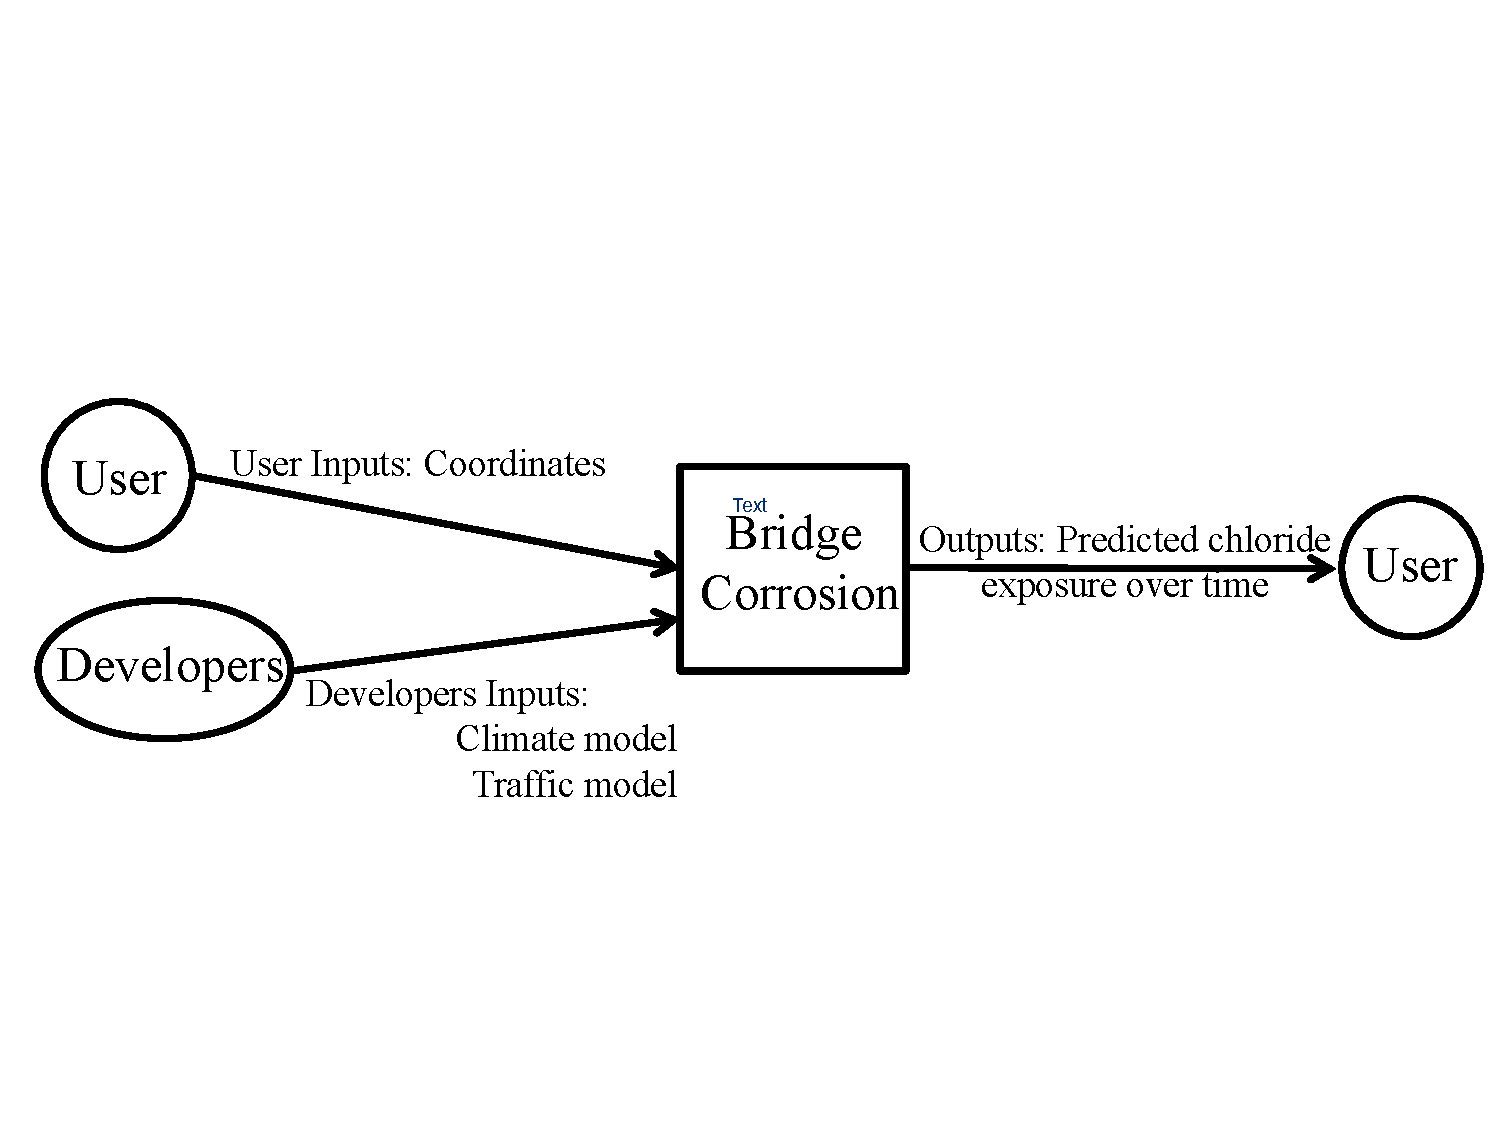
\includegraphics[width=0.8\textwidth]{SystemContextFigure}
\caption{System Context}
\label{Fig_SystemContext} 
\end{center}
\end{figure}


Figure \ref{Fig_SystemContext} shows the system context of the software. The user should input a valid  salt application rate, bridge component and bridge site (coordinates) to the software, and the software will return the predicted chloride exposure in the past and future to the user. The user and the software assume the following responsibilities:

\begin{itemize}
\item User Responsibilities:
\begin{itemize}
\item Provide valid salt application rate, bridge component and bridge site (coordinates) to the software.
\end{itemize}

\item Developer Responsibilities:
\begin{itemize}
\item Provide valid climate table and traffic table to the software.
\end{itemize}

\item BCEP Responsibilities:
\begin{itemize}
\item Build a database storing the chloride exposure data for every GRID\_SIZE grid in the past and future.
\item Search and return the chloride exposure trend of the bridge component in given salt application rate at given input bridge site (coordinate).
\item Provide visualization (line graphs and grids) displaying the output data.
\end{itemize}
\end{itemize}

\subsection{User Characteristics} \label{SecUserCharacteristics}
The end user of BCEP should have a high school understanding of geographic coordinates. Additionally, users may benefit from university level of knowledge of bridge components and chloride-induced corrosion to better understand the context and implications of the predicted chloride exposure.

\subsection{Stakeholders} \label{Stakeholders}
 A stakeholder is a person, group or organization with a vested interest in the project. For BCEP, the stakeholders include:

\begin{itemize}
\item Government agency: Government entities need this data for effective bridge management. By identifying bridges with higher corrosion risks, they can allocate budgets more efficiently.
\item Bridge engineer: Bridge engineers require the accurate data to use as a reference for planning the road construction of JURISDICTION. For example, they need the data to perform analysis and determining the minimum requirements for a bridge to stand for certain years. 
\item Researcher: Professionals within the civil engineering field who are concerned with the impacts of climate change on corrosion damage. In particular, this project is conducted in collaboration with Dr.\ Cancan Yang and Ph.D. candidate Mingsai Xu from the Department of Civil Engineering at McMaster University.
\item Developer: Individuals involved in the development, maintenance, and potential future enhancements of the predictive model. This group may include software developers or engineers tasked with inheriting, sustaining, and advancing the model beyond the initial research phase.
\item Casual user: People that are interested in the bridge chloride exposure of their area and those interest in the impacts of climate change and traffic pattern. 
\end{itemize}


\subsection{System Constraints}
There is no system constraints for this software.
  
\section{Specific System Description}

This section first presents the problem description, which gives a high-level
view of the problem to be solved.  This is followed by the solution characteristics
specification, which presents the assumptions, theories, definitions and finally
the instance models.  

\subsection{Problem Description} \label{Sec_pd}
This project is intended to investigate how climate and traffic might impact corrosion-induced damage for reinforced concrete bridges by influencing their chloride exposure.

\subsubsection{Terminology and  Definitions}
This subsection provides a list of terms that are used in the subsequent
sections and their meaning, with the purpose of reducing ambiguity and making it
easier to correctly understand the requirements.

\begin{itemize}
\item Mass Flow Rate (MFR): The amount of water displaced by a single tire. (kg/s)
\item Spray density: Spray density is the measure of how closely packed the droplets or particles are within the spray plume. It quantifies the amount of material dispersed per unit area. In this document, it is referring to the density of water in the air (mass of water per unit volume of air) in the environment. (\si{kg/m^3})
\item Spray: When water droplets, generally less that 0.5 mm (0.02 inches) in diameter and suspended in the air, are formed after water has impacted a smooth surface and been atomized.
\item Splash: The mechanical action of a vehicle’s tire forcing water out of its path. Splash is generally defined as water drops greater than 1.0 mm (0.04 inches) in diameter, which follow a ballistic path away from the tire.
\item Airborne deposition: The process of chloride ions moving from the atmosphere to solid surfaces.
\item Deposition rate: The rate at which chloride ions are deposited onto a surface over a specific period of time. (\si{kg/m^3})
\item Drainage: The process by which water or other liquids flow away from an area with excess water.
\item AADT: The average daily traffic volume at a given location over an entire year, measured by the number of vehicles.
\item AADTT: The average daily truck traffic volume at a given location over an entire year, measured by the number of vehicles.
\item Pier: An upright support for a structure or superstructure such as an arch or bridge. A bridge pier is a type of structure that extend to the ground below.
\item Deck: The surface of a bridge.

\end{itemize}

\subsubsection{Physical System Description} \label{sec_phySystDescrip}


The key physical system of BCEP, as shown in Figure \ref{4mechanism}, simulate the situation where a vehicle sprays and splashes the water. It includes the following elements:

\begin{itemize}

\item[PS1:] Capillary adhesion: The absorption of water (present on the road surface) by the tires through surface tension.

\item[PS2:] Tread pickup: Water within the grooves of a tire being sprayed and splashed behind the tire by turbulent flow in the grooves.

\item[PS3:] Bow wave: Water sent towards the front of the tire because of the physical displacement of water from the road surface due to the vehicle tires.

\item[PS4:] Side wave: Water sent in the direction perpendicular to the traffic because of the physical displacement of water from the road surface due to the vehicle tires.

\end{itemize}


\begin{figure}[h!]
\begin{center}
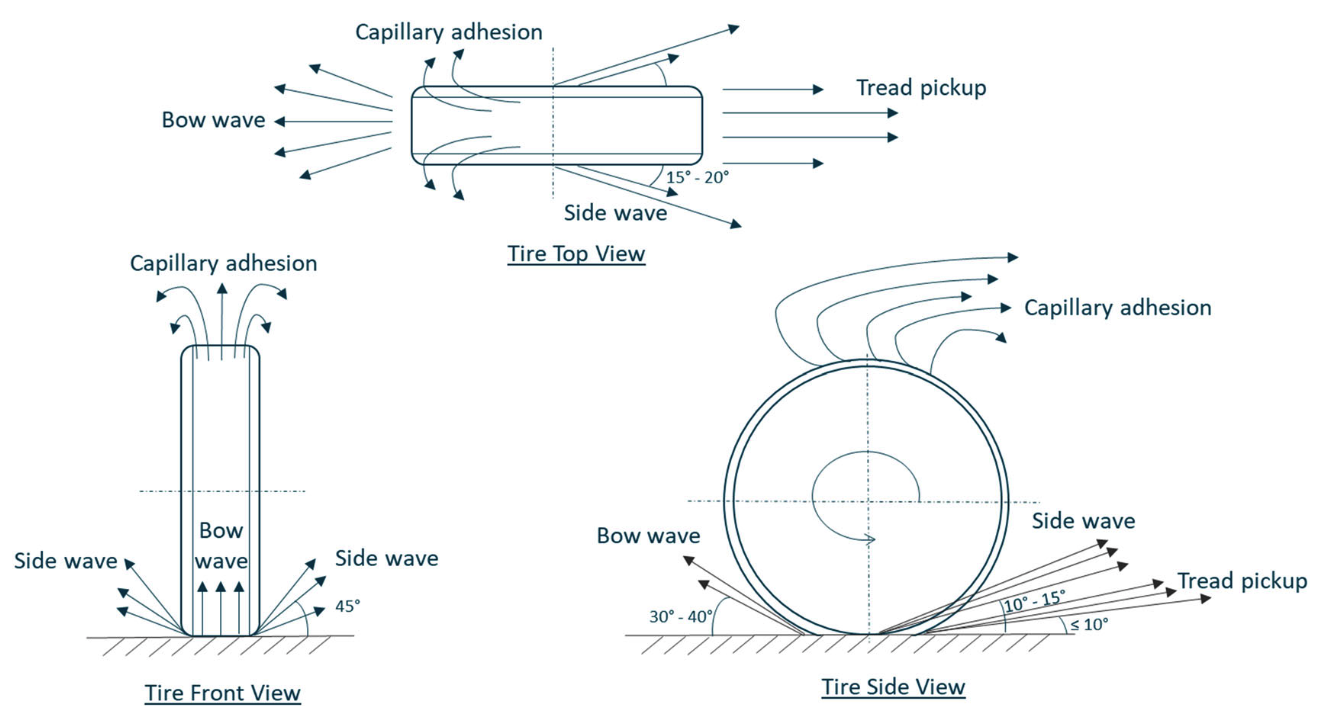
\includegraphics[width=0.9\textwidth]{phymodel}
\caption{\label{4mechanism} Mechanisms of vehicle spray and splash [\reref{ref4}]}

\end{center}
\end{figure}

\newpage
\subsubsection{Goal Statements}

\noindent Given the climate data, traffic data, salt application rate, bridge component and geographical coordinates, the goal is to:

\begin{itemize}

\item[GS\refstepcounter{goalnum}\thegoalnum \label{G_ChlorideExposurePrediction}:] Predict the chloride exposure for bridges in JURISDICTION in the past and future.
\end{itemize}

\subsection{Solution Characteristics Specification}
Section~\ref{sec_assumpt} begins with reasonable assumptions that simplify the original problem. Section~\ref{sec_theoretical} and Section~\ref{sec_gendef} present the theoretical models and general definitions being refined by the instance models, respectively. Section~\ref{sec_datadef} includes the symbols and equations provided for the problem, while Section~\ref{sec_instance} describes the instance models that govern this project. A figure showing the relations between Theoretical Model [TM], General Definition [GD], Data Definition [DD], Instance Model [IM] could be found in Figure \ref{Fig_TraceabilityBetweenModels}.

\subsubsection{Scope Decisions}
Only the damage due to the chloride from deicing salt is considered; other sources of damage, like car accident and mechanical wear, are not considered.

% \plt{This section is optional.}
\subsubsection{Assumptions} \label{sec_assumpt}

This section simplifies the original problem and helps in developing the
theoretical model by filling in the missing information for the physical system.
The numbers given in the square brackets refer to the Theoretical Model [TM],
General Definition [GD], Data Definition [DD], Instance Model [IM], or Likely
Change [LC], in which the respective assumption is used.

\begin{itemize}
\item[A\refstepcounter{assumpnum}\theassumpnum \label{A_dissolve}:] All the deicing salts are dissolved in the water on the road surface.

\item[A\refstepcounter{assumpnum}\theassumpnum \label{A_buildup}:] There is no buildup of chloride ions at the surface over multiple seasons.

\item[A\refstepcounter{assumpnum}\theassumpnum \label{A_pier}:] Only the pier section at the substructure base is affected by the vehicle spray and splash.

\item[A\refstepcounter{assumpnum}\theassumpnum \label{A_deicingSalts}:] All the deicing salts are applied on days with snowfall. (RefBy: \ddref{DD_DSQ})

\item[A\refstepcounter{assumpnum}\theassumpnum \label{A_laneWidth}:] The lane width for all the roads are the same. (RefBy: \ddref{DD_DSQ}, \lcref{LC_laneWidth})

\item[A\refstepcounter{assumpnum}\theassumpnum \label{A_NaCl}:] The main component of deicing salt is NaCl. (RefBy: \ddref{DD_SDTCL})

\item[A\refstepcounter{assumpnum}\theassumpnum \label{A_tireWidth}:] The tire width for all the vehicles are the same. (RefBy: \tref{T_MFRG},  \dref{D_MRCA} -- \dref{D_SDSW})

\item[A\refstepcounter{assumpnum}\theassumpnum \label{A_Speed}:] The speed for all the vehicles are the same, taken as the highway speed limit. (RefBy: \tref{T_MFRG}, \dref{D_MRCA} -- \dref{D_SDSW})

\item[A\refstepcounter{assumpnum}\theassumpnum \label{A_LinearGrowthTraffic}:]  All highway segments has a linear annual growth rate of $r$ AADT and AADTT, with the baseline year being 2006 based on the data from \href{https://icorridor-mto-on-ca.hub.arcgis.com/apps/50798e771bd0440dbc96fd85d8fde9a5/explore}{Ontario Ministry of Transportation}. (RefBy: \ddref{DD_AADT}, \ddref{DD_AADTT})

\item[A\refstepcounter{assumpnum}\theassumpnum \label{A_Data}:] The climate and traffic is constant over the entire area of each GRID\_SIZE cell. (RefBy: \iref{I_DFSB})

\item[A\refstepcounter{assumpnum}\theassumpnum \label{A_Calibration}:] The calibration factor $\alpha$ and $\beta$ are assumed to be 0.5, in the calculation for mass flow rate of bowl waves and side waves. (RefBy: \dref{D_MRBWSW})

\item[A\refstepcounter{assumpnum}\theassumpnum \label{A_deicingSaltsDeposition}:] The deposition of deicing salts along a highway in Sweden is similar to other JURISDICTION. (RefBy: \iref{I_COTS})

\item[A\refstepcounter{assumpnum}\theassumpnum \label{A_fourMechanisms}:] The amount of water is enough to activate all four kinds of mechanisms of vehicle spray and splash. (RefBy: \dref{D_MRCA}, \dref{D_MRTP}, \dref{D_MRBWSW})

\end{itemize}

\subsubsection{Theoretical Models}\label{sec_theoretical}
This section focuses on the general equations and laws the project is based on. 
\newline
\noindent

%TM1
\noindent
\begin{minipage}{\textwidth}
\renewcommand*{\arraystretch}{1.5}
\begin{tabular}{| p{\colAwidth} | p{\colBwidth}|}
\hline
\rowcolor[gray]{0.9}
Number& TM\refstepcounter{theorynum}\thetheorynum \label{T_WFT}\\
\hline
Label &\bf Water film thickness\\
\hline
% Units&$MLt^{-3}T^0$\\
% \hline
SI Units&\si{m}\\
\hline
Equation& $\mathit{WD} = 6 \times 10^{-4} \cdot T^{0.09} (L \cdot I)^{0.6} \cdot S^{-0.33} $\\
\hline
Description & 
The above equation computes the water film thickness (WD) based on the rainfall intensity and pavement surface properties.
\begin{itemize}

\item $\mathit{WD}$ is the water depth. (m)

\item $T$ is the pavement texture. (mm)

\item $L$ is the pavement drainage length. (m)

\item $I$ is the rainfall intensity. (m/h)

\item $S$ is the slope. (m/m)


\end{itemize}

\\
\hline
  Source & [\reref{ref5}] \\
  \hline
  Ref.\ By & \tref{T_MFRG} \\
  \hline
\end{tabular}

\end{minipage}\\


%TM2
\noindent
\begin{minipage}{\textwidth}
\renewcommand*{\arraystretch}{1.5}
\begin{tabular}{| p{\colAwidth} | p{\colBwidth}|}
\hline
\rowcolor[gray]{0.9}
Number& TM\refstepcounter{theorynum}\thetheorynum \label{T_MFRG}\\
\hline
Label &\bf Max flow rate general \\
\hline
% Units&$MLt^{-3}T^0$\\
% \hline
SI Units&\si{kg\per s}\\
\hline
Equation& $\mathit{MR_W} = V \cdot b \cdot \mathit{WD} \cdot \rho_{water} $\\

\hline
Description & 
The above equation ($\mathit{MR_W}$) is the general equation for mass flow rate (MFR), which is the maximum amount of water available for splash and spray.
\begin{itemize}

\item $V$ is the truck speed. (m/s)

\item $b$ is the tire width. (m)

\item $\mathit{WD}$ is the water depth/thickness. (m)

\item $\rho_{water}$ is the density of water. (\si{kg/m^{3}})

\end{itemize}
\\
\hline

  Note & $b$, the tire width, is assumed to be the same for all vehicles according to \aref{A_tireWidth}. $V$, the truck speed, is assumed to be the same for all vehicles, taken as the highway speed limit in Table \ref{TblConstants}, according to \aref{A_Speed}. $\mathit{WD}$, the result of \tref{T_WFT}, is used as a parameter in this equation.\\
  \hline

  Source & [\reref{ref5}] \\
  \hline
  Ref.\ By & \dref{D_MRCA}, \dref{D_MRTP}, \dref{D_MRBWSW}\\ 
  \hline
  Uses\ & \aref{A_tireWidth}, \aref{A_Speed}, \tref{T_WFT}\\
  \hline
\end{tabular}

\end{minipage}\\

%TM3
\noindent
\begin{minipage}{\textwidth}
\renewcommand*{\arraystretch}{1.5}
\begin{tabular}{| p{\colAwidth} | p{\colBwidth}|}
  \hline
  \rowcolor[gray]{0.9}
  Number& TM\refstepcounter{theorynum}\thetheorynum \label{T_CSASG}\\
  \hline
  Label& \bf Chloride sprayed and splashed \\
\hline
% Units&$MLt^{-3}T^0$\\
% \hline
SI Units&\si{kg\per\metre^3} \\
\hline
Equation & $C_{{s}_{air}} = (\mathit{SD_{total\_cl}} \times \frac{1}{\Theta} \times \frac{ADT-N}{N_{lane}}+ \mathit{SD_{total\_cl}} \times \frac{N}{N_{lane}}) \times t_2$ \\
  \hline
  Description& The above equation computes the mass of chloride ions per unit air volume sprayed and splashed ($C_{{s}_{air}}$) by all the vehicles passing near the bridge pier every winter, accounting for all the days with snow in a typical winter season.
  
\begin{itemize}

\item $\mathit{SD_{total\_cl}}$ is the mass of chloride ions per unit air volume, calculated in \ddref{DD_SDTCL}. (\si{kg/m^3})

\item $\Theta$ is the ratio of chloride ions sprayed and splashed by trucks to light-duty vehicles, it is a constant in Table \ref{TblConstants}. 

\item $ADT$ is the average daily traffic. (number of vehicles/day)

\item $N$ is the average number of heavy-duty vehicles per day. (number of vehicles/day)

\item $N_{lane}$ is the number of lanes.

\item $t_2$ is the number of days with snow melting.

\end{itemize}


\\
\hline
Notes & The first part in the parentheses calculate the chloride exposure by light-duty vehicle, and the second part is for heavy-duty vehicles. The calculation focus on the road lane that is closest to the bridge component, so $N_{lane}$ is included in the denominator, to turn the total traffic for the road into traffic for one lane.
\\
\hline
  Source & [\reref{ref4}] \\
  \hline
  Ref.\ By & \dref{D_CSAS} \\ 
  \hline
  Uses \ & \ddref{DD_SDTCL}  \\
  \hline
\end{tabular}
\end{minipage}\\

%TM4
\noindent
\begin{minipage}{\textwidth}
\renewcommand*{\arraystretch}{1.5}
\begin{tabular}{| p{\colAwidth} | p{\colBwidth}|}
  \hline
  \rowcolor[gray]{0.9}
  Number& TM\refstepcounter{theorynum}\thetheorynum \label{T_TAD}\\
  \hline
  Label& \bf  Total airborne deposition at a certain distance \\
\hline
% Units&$MLt^{-3}T^0$\\
% \hline
SI Units&\si{kg\per\metre^3} \\
\hline
Equation & $D(x) = a_{spray} \times e^{-0.05x} + a_{splash} \times e^{-0.5x} $\\ 
  \hline
  Description& The above equation describes the total airborne deposition $D$ at a certain distance $x$ from the road.

\begin{itemize}

\item $a_{spray}$ is the maximum deposition rates that occur from spray. (\si{kg/m^3})

\item $a_{splash}$ is the maximum deposition rates that occur from splash. (\si{kg/m^3})

\item $x$ is the distance between the road and the object. (m)

\end{itemize}


\\
\hline
  Source & [\reref{ref12}] \\
  \hline
  Ref.\ By & \iref{I_COTS} \\ 
  \hline
\end{tabular}
\end{minipage}\\

\subsubsection{General Definitions}\label{sec_gendef}
This section collects the laws and equations that will be used in building the
instance models.

\noindent
\begin{minipage}{\textwidth}
\renewcommand*{\arraystretch}{1.5}
\begin{tabular}{| p{\colAwidth} | p{\colBwidth}|}
\hline
\rowcolor[gray]{0.9}
Number& GD\refstepcounter{defnum}\thedefnum \label{D_MRCA}\\
\hline
Label &\bf Mass flow rate for capillary adhesion\\
\hline
% Units&$MLt^{-3}T^0$\\
% \hline
SI Units&\si{kg\per s}\\
\hline
Equation& 
     $\mathit{MR_{CA}} = V_{speed} \times b \times K \times h_{film} \times \rho_{water}$
  \\
\hline
Description & This equation compute the contribution to the amount of water displaced by a single tire (MFR) of capillary adhesion mechanism ($\mathit{MR_{CA}}$).

\begin{itemize}

\item $V_{speed} $ is the heavy vehicle speed, it is a constant in Table \ref{TblConstants}. (\si{km/h})

\item $b$ is the tire width, it is a constant in Table \ref{TblConstants}. (m)

\item $K$ is the ratio of the tire width that is not a groove to the tire width, it is a constant in Table \ref{TblConstants}. 

\item $h_{film}$ is the depth of the water film picked up in each rotation, it is a constant in Table \ref{TblConstants}. (m)

\item $\rho_{water}$ is the density of water, it is a constant in Table \ref{TblConstants}. (\si{kg/m^{3}})

\end{itemize}
\\
\hline
Notes & This equation is a refinement of \tref{T_MFRG}, it assumes that all vehicles have the same speed and same tire width, as stated in \aref{A_tireWidth} and \aref{A_Speed} \\
\hline
  Source & [\reref{ref4}] \\
  \hline
  Ref.\ By & \dref{D_SDCA} \\ 
  \hline
  Uses\ &  \aref{A_tireWidth}, \aref{A_Speed}, \aref{A_fourMechanisms}, \tref{T_MFRG}\\
  \hline
\end{tabular}
\end{minipage}\\


\subsubsection*{Detailed derivation of mass flow rate for capillary adhesion}

The following derivation is based on the theories purposed in [\reref{ref4}].\\
The maximum mass flow rate associated with capillary adhesion ($\mathit{MR_{CA}}$) is estimated as the number of tire rotations per second multiplied by the volume of water dispersed on each tire rotation multiplied by the density of water, or
 \[ 
\mathit{MR_{CA}} = \left[\frac{V_{speed}}{2\pi R}\right] \cdot \left[ 2\pi R \times b \times K \times h_{film} \right] \times \rho_{water} = \left[V_{speed} \times b \times K \times h_{film} \right] \times  \rho_{water} 
\]
\\

\noindent
\begin{minipage}{\textwidth}
\renewcommand*{\arraystretch}{1.5}
\begin{tabular}{| p{\colAwidth} | p{\colBwidth}|}
\hline
\rowcolor[gray]{0.9}
Number& GD\refstepcounter{defnum}\thedefnum \label{D_MRTP}\\
\hline
Label &\bf Mass flow rate for tread pickup\\
\hline
% Units&$MLt^{-3}T^0$\\
% \hline
SI Units&\si{kg\per s}\\
\hline
Equation& 
      $\mathit{MR_{TP}} = V_{speed} \times b \times (1-K) \times h_{app} \times \rho_{water}$
  \\
\hline
Description & The above equation computes the contribution to the amount of water displaced by a single tire (MFR) of tread pickup mechanism ($\mathit{MR_{TP}}$). 

\begin{itemize}

\item $V_{speed} $ is the heavy vehicle speed, it is a constant in Table \ref{TblConstants}. (km/h)

\item $b$ is the tire width, it is a constant in Table \ref{TblConstants}. (m)

\item $K$ is the ratio of the tire width that is not a groove to the tire width, it is a constant in Table \ref{TblConstants}.

\item $h_{app}$ is the thickness of melted water per day with snow melting. (m)

\item $\rho_{water}$ is the density of water, it is a constant in Table \ref{TblConstants}. (\si{kg/m^{3}})

\end{itemize}

\\
\hline
Notes & This equation is a refinement of \tref{T_MFRG}, it assumes that all vehicle have same speed and tire width, as stated in \aref{A_tireWidth}, \aref{A_Speed}. It also uses $h_{app}$, which is the result calculated from \ddref{DD_DWFT}. As stated in \aref{A_fourMechanisms}, this equation will always be activated as the amount of water is enough.\\
\hline
  Source & [\reref{ref4}] \\
  \hline
  Ref.\ By & \dref{D_SDTP} \\ % \ddref{dsq}, \ddref{dwft}\\
  \hline
  Uses\ & \aref{A_tireWidth}, \aref{A_Speed}, \aref{A_fourMechanisms}, \tref{T_MFRG}, \ddref{DD_DWFT}\\
  \hline
\end{tabular}

\end{minipage}\\



\subsubsection*{Detailed derivation of mass flow rate for tread pickup}


After capillary action, the tire is able to displace a volume of water within its tread. The maximum flow rate for this mechanism ($\mathit{MR_{TP}}$) will occur when all the water contained in the tread volume is flung out of the tread during each tire rotation. Thus, it can be computed as the number of tire rotations per second multiplied by the capacity of the tire’s tread on each rotation multiplied by the density of water:
 \[ 
\mathit{MR_{TP}} = V_{speed} \times b \times (1-K) \times h_{app} \times \rho_{water} 
\]
\\




\noindent
\begin{minipage}{\textwidth}
\renewcommand*{\arraystretch}{1.5}
\begin{tabular}{| p{\colAwidth} | p{\colBwidth}|}
\hline
\rowcolor[gray]{0.9}
Number& GD\refstepcounter{defnum}\thedefnum \label{D_MRBWSW}\\
\hline
Label &\bf Mass flow rate for bow waves and side waves\\
\hline
% Units&$MLt^{-3}T^0$\\
% \hline
SI Units&\si{kg\per s}\\
\hline
Equation& $\mathit{MR_{BW}} = MR_{SW} = 0.5 \times V_{speed} \times b \times (h_{app} - K \times h_{film} - (1-K) \times h_{app}) \times \rho_{water} $ \\
\hline
Description & The above equation computes the contribution to the amount of water displaced by a single tire (MFR) of bow waves mechanism ($\mathit{MR_{BW}}$) and side waves mechanism ($\mathit{MR_{SW}}$). 
\begin{itemize}

\item $V_{speed} $ is the heavy vehicle speed, it is a constant in Table \ref{TblConstants}. (km/h)

\item $b$ is the tire width, it is a constant in Table \ref{TblConstants}. (m)

\item $K$ is the ratio of the tire width that is not a groove to the tire width, it is a constant in Table \ref{TblConstants}.

\item $h_{film}$ is the depth of the water film picked up in each rotation, it is a constant in Table \ref{TblConstants}. (m)

\item $h_{app}$ is the thickness of melted water per day with snow melting. (m)

\item $\rho_{water}$ is the density of water, it is a constant in Table \ref{TblConstants}. (\si{kg/m^{3}})

\end{itemize}
\\
\hline
Notes & This equation is a refinement of \tref{T_MFRG}, it assumes that all vehicle have same speed and tire width, as stated in \aref{A_tireWidth}, \aref{A_Speed}. It also uses $h_{app}$, which is the result calculated from \ddref{DD_DWFT}. The calibration factor $\alpha$ and $\beta$ are assumed to be 0.5, according to \aref{A_Calibration}. As stated in \aref{A_fourMechanisms}, this equation will always be activated as the amount of water is enough.\\
\hline
  Source & [\reref{ref4}] \\
  \hline
  Ref.\ By & \dref{D_SDBW},  \dref{D_SDSW} \\ % \ddref{dsq}, \ddref{dwft}\\
  \hline
  Uses\ & \aref{A_tireWidth}, \aref{A_Speed}, \aref{A_Calibration}, \aref{A_fourMechanisms}, \tref{T_MFRG}, \ddref{DD_DWFT}\\
  \hline
\end{tabular}

\end{minipage}\\


\subsubsection*{Detailed derivation of mass flow rate for bow waves and side waves}

Any remaining water for which there is no capacity either underneath the tire contact area or within the tire tread must be displaced to the front of the tire or to the side, causing the bow wave and side wave, respectively. So, the total mass flow rate that can be attributed to bow and side wave mechanisms can be written as:
 \[ 
\mathit{MR_{BW} + MR_{SW}} =  \rho_{water} \times b \times V_{speed} \times (h_{app} - K \times h_{film} - (1-K) \times h_{app}) \]
\\
So, $\mathit{MR_{BW}}$ and $\mathit{MR_{SW}}$ can be estimated separately as:
 \[ 
\mathit{MR_{BW}} =  \alpha \times \rho_{water} \times b \times V_{speed} \times (h_{app} - K \times h_{film} - (1-K) \times h_{app}) \]
 \[
\mathit{MR_{SW}} = \beta \times \rho_{water} \times b \times V_{speed} \times (h_{app} - K \times h_{film} - (1-K) \times h_{app}) \]
\\
where $\alpha$ and $\beta$ are calibration factors that satisfy $\alpha + \beta = 1$. Until other evidence is available, it will be assumed that $\alpha = \beta = 0.5$.


\newpage

\noindent
\begin{minipage}{\textwidth}
\renewcommand*{\arraystretch}{1.5}
\begin{tabular}{| p{\colAwidth} | p{\colBwidth}|}
\hline
\rowcolor[gray]{0.9}
Number& GD\refstepcounter{defnum}\thedefnum \label{D_SDCA}\\
\hline
Label &\bf Spray density for capillary adhesion \\
\hline
% Units&$MLt^{-3}T^0$\\
% \hline
SI Units&\si{kg\per\metre^3}\\
\hline
Equation&
     $\mathit{SD_{CA}} = (-2.69 \times 10^{-5} \times V' + 2.43 \times 10^{-3}) \times \mathit{MR_{CA}} $
\\
\hline
Description & Spray density is derived by conducting regression analysis to develop relationship between spray density, mass flow rate and vehicle speed, to compute the concentration of water kicked up to the environment. The detailed process could be found in section 6.6.1 in [\reref{ref4}] .
\begin{itemize}

\item $V'$ is the heavy vehicle speed according to \aref{A_Speed}, it is a constant in Table \ref{TblConstants} . (miles/h)

\item $\mathit{MR_{CA}}$ is the mass flow rate for capillary adhesion, calculated by  \dref{D_MRCA}. (kg/s)
\end{itemize}

\\
\hline
  Source & [\reref{ref4}] \\
  \hline
  Ref.\ By & \ddref{DD_TSD} \\
  \hline
  Uses \ & \aref{A_Speed}, \dref{D_MRCA} \\
  \hline
\end{tabular}
\end{minipage}\\


\noindent
\begin{minipage}{\textwidth}
\renewcommand*{\arraystretch}{1.5}
\begin{tabular}{| p{\colAwidth} | p{\colBwidth}|}
\hline
\rowcolor[gray]{0.9}
Number& GD\refstepcounter{defnum}\thedefnum \label{D_SDTP}\\
\hline
Label &\bf Spray density for tread pickup \\
\hline
% Units&$MLt^{-3}T^0$\\
% \hline
SI Units&\si{kg\per\metre^3}\\
\hline
Equation&
      $\mathit{SD_{TP}} = (1.16 \times 10^{-5} \times V' - 5.25 \times 10^{-5}) \times \mathit{MR_{TP}}$ \\    
\hline
Description & Spray density is derived by conducting regression analysis to develop relationship between spray density, mass flow rate and vehicle speed, to compute the concentration of water kicked up to the environment. The detailed process could be found in section 6.6.1 in [\reref{ref4}] .
\begin{itemize}

\item $V'$ is the heavy vehicle speed according to \aref{A_Speed}, it is a constant in Table \ref{TblConstants}. (miles/h)

\item $\mathit{MR_{TP}}$ is the mass flow rate for tread pickup, calculated by  \dref{D_MRTP}. (kg/s)
\end{itemize}

\\
\hline
  Source & [\reref{ref4}] \\
  \hline
  Ref.\ By & \ddref{DD_TSD} \\
  \hline
  Uses \ & \aref{A_Speed}, \dref{D_MRTP} \\
  \hline
\end{tabular}
\end{minipage}\\


\noindent
\begin{minipage}{\textwidth}
\renewcommand*{\arraystretch}{1.5}
\begin{tabular}{| p{\colAwidth} | p{\colBwidth}|}
\hline
\rowcolor[gray]{0.9}
Number& GD\refstepcounter{defnum}\thedefnum \label{D_SDBW}\\
\hline
Label &\bf Spray density for bow waves\\
\hline
% Units&$MLt^{-3}T^0$\\
% \hline
SI Units&\si{kg\per\metre^3}\\
\hline
Equation& $  \mathit{SD_{BW}} = (2.67 \times 10^{-5} \times V' - 4.71 \times 10^{-4}) \times \mathit{MR_{BW}} $
\\
\hline
Description & Spray density is derived by conducting regression analysis to develop relationship between spray density, mass flow rate and vehicle speed, to compute the concentration of water kicked up to the environment. The detailed process could be found in section 6.6.1 in [\reref{ref4}] .
\begin{itemize}

\item $V'$ is the heavy vehicle speed according to \aref{A_Speed}, it is a constant in Table \ref{TblConstants}. (miles/h)

\item $\mathit{MR_{BW}}$ is the mass flow rate for bow waves, calculated by  \dref{D_MRBWSW}. (kg/s)
\end{itemize}

\\
\hline
  Source & [\reref{ref4}] \\
  \hline
  Ref.\ By & \ddref{DD_TSD} \\
  \hline
  Uses \ & \aref{A_Speed}, \dref{D_MRBWSW} \\
  \hline
\end{tabular}
\end{minipage}\\


\noindent
\begin{minipage}{\textwidth}
\renewcommand*{\arraystretch}{1.5}
\begin{tabular}{| p{\colAwidth} | p{\colBwidth}|}
\hline
\rowcolor[gray]{0.9}
Number& GD\refstepcounter{defnum}\thedefnum \label{D_SDSW}\\
\hline
Label &\bf Spray density for side waves \\
\hline
% Units&$MLt^{-3}T^0$\\
% \hline
SI Units&\si{kg\per\metre^3}\\
\hline
Equation& $\mathit{SD_{SW}} = (1.65 \times 10^{-5} \times V' - 3.99 \times 10^{-4}) \times \mathit{MR_{SW}}$
\\
\hline
Description & Spray density is derived by conducting regression analysis to develop relationship between spray density, mass flow rate and vehicle speed, to compute the concentration of water kicked up to the environment. The detailed process could be found in section 6.6.1 in [\reref{ref4}] .
\begin{itemize}

\item $V'$ is the heavy vehicle speed according to \aref{A_Speed}, it is a constant in Table \ref{TblConstants}. (miles/h)

\item $\mathit{MR_{SW}}$ is the mass flow rate for side waves, calculated by  \dref{D_MRBWSW}. (kg/s)

\end{itemize}

\\
\hline
  Source & [\reref{ref4}] \\
  \hline
  Ref.\ By & \ddref{DD_TSD} \\
  \hline
  Uses \ & \aref{A_Speed}, \dref{D_MRBWSW} \\
  \hline
\end{tabular}
\end{minipage}\\


\noindent
\begin{minipage}{\textwidth}
\renewcommand*{\arraystretch}{1.5}
\begin{tabular}{| p{\colAwidth} | p{\colBwidth}|}
  \hline
  \rowcolor[gray]{0.9}
  Number& GD\refstepcounter{defnum}\thedefnum \label{D_CSAS}\\
  \hline
  Label& \bf Chloride sprayed and splashed \\
\hline
% Units&$MLt^{-3}T^0$\\
% \hline
SI Units&\si{kg\per\metre^3}\\
  \hline
  Equation & $C_{s_{air}} = (\mathit{SD_{total\_cl}} \times \frac{1}{\Theta} \times (AADT - AADTT) + SD_{total\_cl} \times AADTT) \times t_2$ \\
  \hline
  Description& This equation refines \tref{T_CSASG}. The cumulative mass of chloride ions per unit air volume sprayed and splashed by all vehicles every winter, can be calculated by first finding the mass of chloride ions per unit air volume sprayed and splashed by all the vehicles per day, and times with the number of days with snow melting.
  
\begin{itemize}

\item $\mathit{SD_{total~cl}}$ is the mass of chloride ions per unit air volume, it is the result of \ddref{DD_SDTCL}. (\si{kg/m^3})

\item $\Theta$ is the ratio of chloride ions sprayed and splashed by trucks to light-duty vehicles, it is a constant in Table \ref{TblConstants}.

\item $AADT$ is the annual average daily traffic per lane, given by traffic table \ddref{DD_AADT}.

\item $AADTT$ is the annual average daily truck traffic per lane, given by traffic table \ddref{DD_AADTT}.

\item $t_2$ is the number of days with snow melting, given by climate table in \ddref{DD_t2}.
\end{itemize}
\\
  \hline
  Sources & [\reref{ref7}, \reref{ref8}] \\
  \hline
  Ref.\ By & \iref{I_COTS} \\
  \hline
  Uses \ &  \tref{T_CSASG} , \ddref{DD_AADT}, \ddref{DD_AADTT}, \ddref{DD_t2}, \ddref{DD_SDTCL}\\
  \hline
\end{tabular}
\end{minipage}\\

\subsubsection{Data Definitions}\label{sec_datadef}
This section collects and defines all the data needed to build the instance
models. The dimension of each quantity is also given.  
~\newline


\noindent
\begin{minipage}{\textwidth}
\renewcommand*{\arraystretch}{1.5}
\begin{tabular}{| p{\colAwidth} | p{\colBwidth}|}
\hline
\rowcolor[gray]{0.9}
Number& DD\refstepcounter{datadefnum}\thedatadefnum \label{DD_AADT}\\
\hline
Label& \bf AADT\\
\hline
Symbol & $AADT$\\
\hline
  SI Units & N/A\\
  \hline
 Equation & $AADT:\mathbb{R} \times \mathbb{R} \rightarrow \mathbb{R} $\\
  \hline
  Description & $AADT(longitude, latitude)$ is the Annual Average Daily Traffic as a function of position, it is determined from the traffic table by taking two real number (longitude and latitude), and return a real number (AADT). An example of it could be found in Table \ref{Table:AADT}). The traffic data is constant over each GRID\_SIZE cell by \aref{A_Data}. According to \aref{A_LinearGrowthTraffic}, $AADT$ has a linear growth rate of $r$ with the baseline year being 2006. Future $AADT$ values are determined using this growth rate. 

  \\
  \hline
  Sources& [\reref{ref7}] \\
  \hline
  Ref.\ By & \dref{D_CSAS}, \iref{I_COTD}   \\
  \hline
   Uses \ &  \aref{A_LinearGrowthTraffic}, \aref{A_Data}\\
  \hline
\end{tabular}
\end{minipage}\\


\noindent
\begin{minipage}{\textwidth}
\renewcommand*{\arraystretch}{1.5}
\begin{tabular}{| p{\colAwidth} | p{\colBwidth}|}
\hline
\rowcolor[gray]{0.9}
Number& DD\refstepcounter{datadefnum}\thedatadefnum \label{DD_AADTT}\\
\hline
Label& \bf AADTT\\
\hline
Symbol & $AADTT$\\
\hline
% Units& $Mt^{-3}$\\
% \hline
  SI Units & N/A\\
  \hline
 Equation & $AADTT: \mathbb{R} \times \mathbb{R} \rightarrow \mathbb{R} $\\
  \hline
  Description & $AADTT(longitude, latitude)$ is the Annual Average Daily Truck Traffic as a function of position, it is determined from the traffic table by taking two real number (longitude and latitude), and return a real number (AADTT). An example of it could be found in Table \ref{Table:AADTT}). The traffic data is constant over each GRID\_SIZE cell by \aref{A_Data}. According to \aref{A_LinearGrowthTraffic}, $AADTT$ has a linear growth rate of $r$ with the baseline year being 2006. Future $AADTT$ values are determined using this growth rate. 
  \\
  \hline
  Sources& [\reref{ref7}] \\
  \hline
  Ref.\ By & \dref{D_CSAS}  \\
  \hline
   Uses \ &  \aref{A_LinearGrowthTraffic}, \aref{A_Data}\\
  \hline
\end{tabular}
\end{minipage}\\


\noindent
\begin{minipage}{\textwidth}
\renewcommand*{\arraystretch}{1.5}
\begin{tabular}{| p{\colAwidth} | p{\colBwidth}|}
\hline
\rowcolor[gray]{0.9}
Number& DD\refstepcounter{datadefnum}\thedatadefnum \label{DD_htotal}\\
\hline
Label& \bf Total snowfall \\
\hline
Symbol & $h_{total}$\\
\hline
% Units& $Mt^{-3}$\\
% \hline
  SI Units & m\\
  \hline
 Equation & $h_{total}: \mathbb{R} \times \mathbb{R} \times \mathbb{N}  \rightarrow \mathbb{R}$\\
  \hline
  Description & $h_{total}(longitude, latitude, year)$ is the total snowfall during a winter season, it is determined from the climate table by taking two real number (longitude and latitude) and one natural number (year), and return a real number ($h_{total}$).  An example of the $h
_{total}$ in climate table could be found in Table \ref{Table:htotal}.
  \\
  \hline
  Sources& [\reref{ref7}] \\
  \hline
  Ref.\ By & \ddref{DD_DSQ}, \ddref{DD_DWFT}, \iref{I_COTD} \\
  \hline
   Uses \ & \aref{A_Data}\\
  \hline
\end{tabular}
\end{minipage}\\


\noindent
\begin{minipage}{\textwidth}
\renewcommand*{\arraystretch}{1.5}
\begin{tabular}{| p{\colAwidth} | p{\colBwidth}|}
\hline
\rowcolor[gray]{0.9}
Number& DD\refstepcounter{datadefnum}\thedatadefnum \label{DD_t1}\\
\hline
Label& \bf Snowfall days \\
\hline
Symbol & $t_1$\\
\hline
% Units& $Mt^{-3}$\\
% \hline
  SI Units & day\\
  \hline
 Equation & $t_1: \mathbb{R} \times \mathbb{R} \times \mathbb{N}  \rightarrow \mathbb{N}$ \\
  \hline
  Description & $t_1(longitude, latitude, year)$ is the number of days with snowfall during a winter season, it is determined from the climate table by taking two real number (longitude and latitude) and one natural number (year), and return a real number ($t_1$). An example of the $t_1$ in climate table could be found in Table \ref{Table:t1}.
  \\
  \hline
  Sources& [\reref{ref7}] \\
  \hline
  Ref.\ By & \ddref{DD_DSQ}   \\
  \hline
   Uses \ & \aref{A_Data}\\
  \hline
\end{tabular}
\end{minipage}\\


\noindent
\begin{minipage}{\textwidth}
\renewcommand*{\arraystretch}{1.5}
\begin{tabular}{| p{\colAwidth} | p{\colBwidth}|}
\hline
\rowcolor[gray]{0.9}
Number& DD\refstepcounter{datadefnum}\thedatadefnum \label{DD_t2}\\
\hline
Label& \bf Snow melting days\\
\hline
Symbol & $t_2$\\
\hline
% Units& $Mt^{-3}$\\
% \hline
  SI Units & day\\
  \hline
 Equation & $t_2: \mathbb{R} \times \mathbb{R} \times \mathbb{N}  \rightarrow \mathbb{N}$\\
  \hline
  Description & $t_2(longitude, latitude, year)$ is the number of days with snow melting during a winter season, it is determined from the climate table by taking two real number (longitude and latitude) and one natural number (year), and return a real number ($t_2$). An example of the $t_2$ in climate table could be found in Table \ref{Table:t2}.
  \\
  \hline
  Sources& [\reref{ref7}] \\
  \hline
  Ref.\ By & \dref{D_CSAS}, \ddref{DD_DWFT}   \\
  \hline
   Uses \ &   \aref{A_Data}\\
  \hline
\end{tabular}
\end{minipage}\\


\noindent
\begin{minipage}{\textwidth}
\renewcommand*{\arraystretch}{1.5}
\begin{tabular}{| p{\colAwidth} | p{\colBwidth}|}
\hline
\rowcolor[gray]{0.9}
Number& DD\refstepcounter{datadefnum}\thedatadefnum \label{DD_DSQ}\\
\hline
Label& \bf Deicing salts quantity\\
\hline
Symbol &$M_{app}$\\
\hline
  SI Units & \si{kg/m^2}\\
  \hline
  Equation& 

     \[M_{app}= \left\{
\begin{aligned}
  & \frac{V_{salt_h} \times h_{total}}{t_1 \times W_{lane}} && \text{for high salt application rate} \\
  & \frac{V_{salt_l} \times h_{total}}{t_1 \times W_{lane}} && \text{for low salt application rate} 
\end{aligned} \right. \]
\\

  \hline
  Description & The equation determine the quantity of deicing salts applied per day with snowfall, according to \aref{A_deicingSalts}, that the deicing salts are applied on the days of snowfall. There are two cases of calculating $M_{app}$, one is for high salt application rate, and the other one is low salt application rate, both taken as constant in Table \ref{TblConstants}.

\begin{itemize}

\item $V_{salt_h}$ is the normalized high salt application rate, it is a constant in Table \ref{TblConstants}. (t/cm/km)
\item $V_{salt_l}$ is the normalized low salt application rate, it is a constant in Table \ref{TblConstants}. (t/cm/km)
\item $h_{total}$ is the total snowfall during a winter season, given by the climate table \ddref{DD_htotal}. (m)

\item $t_{1}$ is the number of days with snowfall, given by the climate table \ddref{DD_t1}.

\item $W_{lane}$ is the lane width. According to \aref{A_laneWidth}, all the lane has the same width, it is a constant in Table \ref{TblConstants}. (m).
\end{itemize}

  \\
  \hline
  Sources& [\reref{ref4}, \reref{ref7}] \\
  \hline
  Ref.\ By & \ddref{DD_RSW}   \\
  \hline
  Uses & \aref{A_deicingSalts}, \aref{A_laneWidth}, \ddref{DD_htotal}, \ddref{DD_t1} \\
  \hline
\end{tabular}
\end{minipage}\\

\noindent
\begin{minipage}{\textwidth}
\renewcommand*{\arraystretch}{1.5}
\begin{tabular}{| p{\colAwidth} | p{\colBwidth}|}
\hline
\rowcolor[gray]{0.9}
Number& DD\refstepcounter{datadefnum}\thedatadefnum \label{DD_DWFT}\\
\hline
Label& \bf Daily water film thickness\\
\hline
Symbol &$h_{app}$\\
\hline
% Units& $Mt^{-3}$\\
% \hline
  SI Units & \si{\meter}\\
  \hline
  Equation&$h_{app} = h_{total}/t_2$\\
  \hline
  Description & The equaition above calculates the thickness of melted water per day with snow melting.
\begin{itemize}

\item $h_{total}$ is the the total snowfall during a winter season, given by the climate table \ddref{DD_htotal}. (m)

\item $t_2$ is the number of days with snow melting, given by the climate table \ddref{DD_t2}.


\end{itemize}

  \\
  \hline
  Sources& [\reref{ref4}, \reref{ref9}] \\
  \hline
  Ref.\ By &  \dref{D_MRTP}, \dref{D_MRBWSW},  \ddref{DD_RSW} \\ 
  \hline
  Uses & \ddref{DD_htotal}, \ddref{DD_t2}\\
  \hline
\end{tabular}
\end{minipage}\\

\noindent
\begin{minipage}{\textwidth}
\renewcommand*{\arraystretch}{1.5}
\begin{tabular}{| p{\colAwidth} | p{\colBwidth}|}
\hline
\rowcolor[gray]{0.9}
Number& DD\refstepcounter{datadefnum}\thedatadefnum \label{DD_TSD}\\
\hline
Label &\bf Total spray density\\
\hline
% Units&$MLt^{-3}T^0$\\
% \hline
SI Units&\si{kg\per m^3}\\
\hline
Equation& $\mathit{SD_{total} = SD_{CA} + SD_{TP} + SD_{BW} + SD_{SW}}$\\
\hline
Description & The spray density (i.e. mass of water per unit air volume kicked up by each passing truck), is the sum of the four mechanism.

\begin{itemize}

\item $\mathit{SD_{CA}}$ is the spray density due to capillary adhesion, calculated by \dref{D_SDCA}.
\item $\mathit{SD_{TP}}$ is the spray density due to tread pickup, calculated by \dref{D_SDTP}.
\item $\mathit{SD_{BW}}$ is the spray density due to bow waves, calculated by \dref{D_SDBW}
\item $\mathit{SD_{SW}}$ is the spray density due to side waves, calculated by \dref{D_SDSW}.

\end{itemize}

\\
\hline
  Source &  [\reref{ref4}] \\
  \hline
  Ref.\ By & \ddref{DD_SDTCL} \\ 
  \hline
  Uses\ & \dref{D_SDCA}, \dref{D_SDTP}, \dref{D_SDBW}, \dref{D_SDSW}\\
  \hline
\end{tabular}

\end{minipage}\\


%ratio of salt over water
\noindent
\begin{minipage}{\textwidth}
\renewcommand*{\arraystretch}{1.5}
\begin{tabular}{| p{\colAwidth} | p{\colBwidth}|}
\hline
\rowcolor[gray]{0.9}
Number& DD\refstepcounter{datadefnum}\thedatadefnum \label{DD_RSW}\\
\hline
Label &\bf Ratio of salt over water \\
\hline
% Units&$MLt^{-3}T^0$\\
% \hline
SI Units&none\\
\hline
Equation & $\delta_{salt} =\frac{M_{app}}{h_{app} \times \rho_{water}}$ \\
\hline
Description & This equation computes the ratio of the mass of salt applied per unit area of road to the mass of water per unit area of road.
\begin{itemize}

\item $M_{app}$ is the quantity of deicing salts applied per day, calculated by \ddref{DD_DSQ}. (\si{kg/m^2})

\item $h_{app}$ is the thickness of melted water per day, calcualted by \ddref{DD_DWFT}. (m)

\item $\rho_{water}$ is the density of water, it is a constant in Table \ref{TblConstants}. (\si{kg/m^{3}}) 
\end{itemize}

\\
\hline
  Source &  [\reref{ref4}]\\
  \hline
  Ref.\ By & \ddref{DD_SDTCL} \\ 
  \hline
  Uses \ &   \ddref{DD_DSQ}, \ddref{DD_DWFT} \\
  \hline
\end{tabular}
\end{minipage}\\

\noindent
\begin{minipage}{\textwidth}
\renewcommand*{\arraystretch}{1.5}
\begin{tabular}{| p{\colAwidth} | p{\colBwidth}|}
\hline
\rowcolor[gray]{0.9}
Number& DD\refstepcounter{datadefnum}\thedatadefnum \label{DD_SDTCL}\\
\hline
Label &\bf Mass of chloride ions \\
\hline
% Units&$MLt^{-3}T^0$\\
% \hline
SI Units&\si{kg\per\metre^3} \\
\hline
Equation & $\mathit{SD_{total\_cl} =SD_{total} \times \delta_{salt} \times \theta_{chloride}}$ \\
\hline
Description & This equation computes the mass of chloride ions per unit air volume kicked up by each truck, where we assume the chloride ions are from NaCl (\aref{A_NaCl}).
\begin{itemize}
\item $\theta_{chloride}$ is the molar mass ratio of chloride to deicing salts, it is a constant in Table \ref{TblConstants}. (ratio)
\item $SD_{total}$ is the mass of water per unit air volume, calculated by \ddref{DD_TSD}. (\si{kg/m^3})

\item $\delta_{salt}$ is the salt-to-water mass ratio per unit area of road, calculated by \ddref{DD_RSW}. (ratio)



\end{itemize}

\\
\hline
  Source &  [\reref{ref4}, \reref{ref7}]  \\
  \hline
  Ref.\ By & \tref{T_CSASG}, \dref{D_CSAS} \\ 
  \hline
  Uses \ & \aref{A_NaCl}, \ddref{DD_TSD}, \ddref{DD_RSW} \\
  \hline
\end{tabular}
\end{minipage}\\



\subsubsection{Instance Models} \label{sec_instance}    
This section transforms the problem defined in Section~\ref{Sec_pd} into 
one which is expressed in mathematical terms. It uses concrete symbols defined 
in Section~\ref{sec_datadef} to replace the abstract symbols in the models 
identified in Sections~\ref{sec_theoretical} and~\ref{sec_gendef}.

The goal \gsref{G_ChlorideExposurePrediction} is solved by \iref{I_COTS}, \iref{I_COTD}, \iref{I_DFSB}.


~\newline


\noindent
\begin{minipage}{\textwidth}
\renewcommand*{\arraystretch}{1.5}
\begin{tabular}{| p{\colAwidth} | p{\colBwidth}|}
  \hline
  \rowcolor[gray]{0.9}
  Number& IM\refstepcounter{instnum}\theinstnum \label{I_COTS}\\
  \hline
  Label& \bf Chloride on the pier \\
  \hline
  Input& $C_{s_{air}}, d$\\
  \hline
  Output& $C_s$ \\
  \hline
  Equation& $C_s = 0.015 \times C_{s_{air}} \times e^{-0.05d} + 0.985 \times C_{s_{air}} \times  e^{-0.5d}$\\ 
  \hline
  Description& The above equation is a refinement of \tref{T_TAD}, it is assumed that the situation in Sweden is similar to other JURISDICTION, so theories in [\reref{ref11}, \reref{ref12}] could be applied. This equation computes the chloride ions deposition on bridge substructure, taking into account the distance between the edge of the road near the bridge substructure and the bridge substructure. 
\begin{itemize}

\item $C_{s_{air}}$ is the result from \dref{D_CSAS}, which is the cumulative mass of chloride ions per unit air volume sprayed and splashed by all the vehicles passing near the bridge pier. (\si{kg/m^3})

\item $d$ is the distance between the road edge and nearby bridge structure, it is a constant in Table \ref{TblConstants}. (m)


\end{itemize}
  \\
  \hline
  Sources& [\reref{ref7}, \reref{ref10}, \reref{ref11}, \reref{ref12}] \\
  \hline
  Ref.\ By & \iref{I_DFSB}, \lcref{LC_SASC}  \\
  \hline
  Uses \ & \aref{A_deicingSaltsDeposition}, \tref{T_TAD}, \dref{D_CSAS} \\
  \hline
\end{tabular}
\end{minipage}\\

\subsubsection*{Detailed derivation of chloride on the surface}
In \tref{T_TAD}, it is mentioned that
\[
C_s = a_{spray} \times e^{-0.05x} + a_{splash} \times e^{-0.5x}\\ 
\]
\\
Given the distance between road edge and nearby bridge structure is $d$, we have: 
\[
C_s = a_{spray} \times e^{-0.05d} + a_{splash} \times e^{-0.5d}\\ 
\]
\\
According to [\reref{ref11}, \reref{ref12}] which measured the deposition of deicing salts along a highway in Sweden to define the relation between the mass of deicing salts per unit area and distance from roadside, and used nonlinear fitting techniques to determine the proportions of sprayed and splashed chloride ions:
\[
a_{spray} = a_{air} \times 0.015
\]
\[
a_{splash} = a_{air} \times 0.985
\]
\\
Combining the above equation in the scenario of chloride, where $a_{air}$ could be substituted as $C_{s_{air}}$, the total maximum chloride deposition rate that can occur:
\[
a_{spray} = C_{s_{air}} \times 0.015
\]
\[
a_{splash} = C_{s_{air}} \times 0.985
\]
\\
then we have:
\[
C_s = 0.015 \times C_{s_{air}} \times e^{-0.05d} + 0.985 \times C_{s_{air}} \times  e^{-0.5d}
\]


~\newline

\noindent
\begin{minipage}{\textwidth}
\renewcommand*{\arraystretch}{1.5}
\begin{tabular}{| p{\colAwidth} | p{\colBwidth}|}
  \hline
  \rowcolor[gray]{0.9}
  Number& IM\refstepcounter{instnum}\theinstnum \label{I_COTD}\\
  \hline
  Label& \bf Chloride on the deck \\
  \hline
  Input& $h_{total}, AADT$\\
  \hline
  Output& $C_s$ \\
  \hline
  Equation& $C_s = 0.11 \times h_{total} - 0.000189 \times AADT + 3.349$\\ 
  \hline
  Description& The above equation computes the chloride ions deposition on bridge decks. It is based on a linear regression model by [\reref{ref6}],  that characterize the relationship between the surface chloride concentration on bridge decks and two key factors: the annual snowfall amount ($h_{total}$) and the AADT

\begin{itemize}

\item $h_{total}$ is the total snowfall during a winter season, given by climate table in \ddref{DD_htotal}. (m)

\item $AADT$ is the annual average daily traffic, given by traffic table in \ddref{DD_AADT}.
\end{itemize}
  \\
  \hline
  Sources& [\reref{ref6}, \reref{ref7}] \\
  \hline
  Ref.\ By & \iref{I_DFSB}  \\
  \hline
  Uses \ & \ddref{DD_AADT}, \ddref{DD_htotal} \\
  \hline
\end{tabular}
\end{minipage}\\


~\newline
\noindent
\begin{minipage}{\textwidth}
\renewcommand*{\arraystretch}{1.5}
\begin{tabular}{| p{\colAwidth} | p{\colBwidth}|}
  \hline
  \rowcolor[gray]{0.9}
  Number& IM\refstepcounter{instnum}\theinstnum \label{I_DFSB}\\
  \hline
  Label& \bf Search data for specific coordinate \\
  \hline
  Input& $long:\mathbb{R},lat:\mathbb{R}$\\
  \hline
  Output & $[C_{s}]_{n}^{m}$ \\
  \hline
  Description & This instance model get the longitude and latitude as input, and return a list of surface chloride concentration, over the time periods $n$ to $m$ as output, which is the result of \iref{I_COTS} and \iref{I_COTD}. The searching process is conducted using coding logic. This is the model that the end user of this software will encounter.

\begin{itemize}

\item $(long, lat)$ is the coordinate of a location. (\degree, \degree)
\item $[C_{s}]_{n}^{m}$ is a list of chloride exposure data over the time periods $n$ to $m$. ([\si{kg/m^3}])
\item $n$ is the start year (an integer) for the period, based on the availability of data in the climate and traffic tables.
\item $m$ is the end year (an integer) for the period, based on the availability of data in the climate and traffic tables.
\end{itemize}
 \\
  \hline
  Uses \ & \aref{A_Data}, \iref{I_COTS}, \iref{I_COTD}
  \\
  \hline
 \end{tabular}
\end{minipage}\\


\subsubsection{Input Data Constraints} \label{sec_DataConstraints}    

Table~\ref{TblInputVar} shows the data constraints on the input output
variables. The column for physical constraints gives the physical limitations
on the range of values that can be taken by the variable. The column for
software constraints restricts the range of inputs to reasonable values. The software constraints will be helpful in the design stage for picking suitable
algorithms.  The constraints are conservative, to give the user of the model the
flexibility to experiment with unusual situations. The column for typical values lists the most frequent occurrences in the traffic and climate table. The uncertainty column
provides an estimate of the confidence with which the physical quantities can be measured. This information would be part of the input if one were performing an uncertainty quantification exercise. In the BCEP project, we talk about not only the input variables mentioned in instance models, but also include those in other models that the instance models use. The physical constraints are purposed by [\reref{ref4}]. Beside those, the input of the software need to be coordinates inside JURISDICTION. This will be done by input checking algorithm later. \\
The specification parameters in Table~\ref{TblInputVar} are listed in
Table~\ref{TblConstants}.

\begin{table}[!h]
  \caption{Input Variables} \label{TblInputVar}
  \renewcommand{\arraystretch}{1.2}
\noindent \begin{longtable*}{l l l l c} 
  \toprule
  \textbf{Var} & \textbf{Physical Constraints} & \textbf{Software Constraints} &
                             \textbf{Typical Value} & \textbf{Uncertainty}\\
  \midrule 
  $AADT$ & $AADT \ge 0$ & $AADT \ge 0$ & 559 & 10\%  \\
  $AADTT$ & $AADTT \ge 0$ & $AADTT \ge 0$ & 103  & 10\%
  \\
  $h_{total}$ & $h_{total} \ge 0$ & $h_{total} \ge 0$ &  70  & 10\%
  \\
  $lat$ & $-90 \leq lat \leq 90$ & $-90 \leq lat \leq 90$ & 48.0863 & 10\%
  \\
  $long$ & $0 \leq long \leq 360$ & $0 \leq long \leq 360$ &  275.0678 & 10\%
  \\
  $t_1$ & $0 \leq t_1 \leq 365$ & $0 \leq t_1 \leq 365$ &  90  & 10\%
  \\
  $t_2$ & $0 \leq t_2 \leq 365$ & $0 \leq t_2 \leq 365$ &  70  & 10\%
  \\
  \bottomrule
\end{longtable*}
\end{table}

\noindent 
\subsubsection{Properties of a Correct Solution} \label{sec_CorrectSolution}

\noindent
A correct solution must exhibit the chloride exposure values that does not exceed the solubility limits of chloride ions, which is according to the \href{https://en.m.wikipedia.org/wiki/Sodium_chloride}{property of sodium chloride}.
\begin{table}[!h]
\caption{Output Variables} \label{TblOutputVar}
\renewcommand{\arraystretch}{1.2}
\noindent \begin{longtable*}{l l} 
  \toprule
  \textbf{Var} & \textbf{Physical Constraints} \\
  \midrule 
  $C_s$ & $C_s < 360 ~ kg/m^3$  \\
  
   \bottomrule
\end{longtable*}
\end{table}

\newpage
\section{Requirements}
This section provides the functional requirements, the business tasks that the
software is expected to complete, and the nonfunctional requirements, the
qualities that the software is expected to exhibit.

\indent 
\subsection{Functional Requirements}

\begin{itemize}
\item[R\refstepcounter{reqnum}\thereqnum \label{R_InputClimate}:] The climate table should be processed by domain expert, originally from the \href{https://climate-modelling.canada.ca/climatemodeldata/canrcm/CanRCM4/index.shtml}{CanRCM4}.
 
\item[R\refstepcounter{reqnum}\thereqnum \label{R_InputTraffic}:] The traffic table should be processed by domain expert, originally from the \href{https://icorridor-mto-on-ca.hub.arcgis.com/apps/50798e771bd0440dbc96fd85d8fde9a5/explore}{AASHTOWare Pavement ME Design Traffic Map}.
\item[R\refstepcounter{reqnum}\thereqnum \label{R_InputMap}:] The software should have a map of JURISDICTION that users can click to provide the input coordinate (longitude \& latitude).

\item[R\refstepcounter{reqnum}\thereqnum \label{R_Inputs}:] The software should only accept coordinate that are inside JURISDICTION. (By \iref{I_DFSB})

\item[R\refstepcounter{reqnum}\thereqnum \label{R_Parameter}:] The software should have an option for user to select parameters for the two bridge components: pier and deck. For chloride on pier (\iref{I_COTS}) consider the different salt application rate (\ddref{DD_DSQ}), while the chloride on deck (\iref{I_COTD}) is not related to salt application rate.

%\item[R\refstepcounter{reqnum}\thereqnum \label{R_Map}:] The result list of chloride exposure rate should be visualized in the map using color scheme to represent the severity of chloride exposure data across different regions.

\item[R\refstepcounter{reqnum}\thereqnum \label{R_OutputInputs}:] The result list of surface chloride concentration should be of precise decimal data, showing the trend of chloride exposure from 2006 to 2100 at the input location. (By \iref{I_DFSB})

\item[R\refstepcounter{reqnum}\thereqnum \label{R_OutputVisualization}:] The result list of surface chloride concentration should have an visualization of line graph and table.

\item[R\refstepcounter{reqnum}\thereqnum \label{R_OutputDownload}:] The result list of surface chloride concentration and the visualization should be able to be downloaded by users to their local machine in csv. 


\end{itemize}


\subsection{Nonfunctional Requirements}

\noindent \begin{itemize}

\item[NFR\refstepcounter{nfrnum}\thenfrnum \label{NFR_Reliability}:]   \textbf{Reliability}: The reliability is measured and verified in the \href{https://github.com/CynthiaLiu0805/BridgeCorrosion/blob/main/docs/VnVPlan/VnVPlan.pdf}{VnVplan}.

\item[NFR\refstepcounter{nfrnum}\thenfrnum \label{NFR_Usability}:] \textbf{Usability}: The software interface should be intuitive and easy to use, allowing users in the section \ref{SecUserCharacteristics} to easily choose salt application levels and concerned bridge components, input coordinates or click on the map, look at the predicted chloride exposure, and download the input data and the results of chloride exposure at that specific location in no more than five minutes. More measurements about usability could be found in \href{https://github.com/CynthiaLiu0805/BridgeCorrosion/blob/main/docs/VnVPlan/VnVPlan.pdf}{VnVplan}.

\item[NFR\refstepcounter{nfrnum}\thenfrnum \label{NFR_Maintainability}:] \textbf{Maintainability}: The code for this software should be designed and structured in a way that it could be easily comprehended and modified by other potential developers, taking only 10\% of the origin develop time.

\item[NFR\refstepcounter{nfrnum}\thenfrnum \label{NFR_Portability}:]  \textbf{Portability}: This software should be able to run on recent versions of Google Chrome, Firefox, MS Edge and Safari. The operating system include Windows 7+ and Mac OS X 10.7+.

\item[NFR\refstepcounter{nfrnum}\thenfrnum \label{NFR_Scalability}:]   \textbf{Scalability}: The software should be scalable to accommodate potential future expansions to more JURISDICTION, support concurrent users while maintaining a quick response time.
\end{itemize}

\subsection{Rationale}

The assumptions made in this document are based on practical considerations to simplify and quantify the data required in the model:
\begin{itemize} 
\item In \aref{A_deicingSalts}, the deicing salts need to be applied on the roads in time to ensure safe driving conditions during winter weather. 
\item \aref{A_laneWidth}, \aref{A_tireWidth} and \aref{A_Speed} simplify the model by standardizing the lane width, tire width and vehicle speed, which streamlines the analysis and allows for consistent calculations.
\item \aref{A_NaCl} simplifies the model while still capturing the essence of typical deicing salt compositions, as NaCl is one of the most widely used deicing salts due to its effectiveness and affordability.
\item It is important to note that the traffic data of the Pavement ME Design Traffic Map was collected in the year of 2006. However, It has been observed that the traffic volume across Ontario experiences an annual growth rate of about $r$ on average, so to account for the time-variant nature of traffic volume and its impact on chloride exposure, a linear annual growth rate of $r$ was applied to both AADT and AADTT for all highway segments in \aref{A_LinearGrowthTraffic}. 
\item \aref{A_Data} is assumed following the resolution of the CanRCM4 model ([\reref{ref13}]), where the climate data are extracted from.

\end{itemize}

The constraints in Table \ref{TblInputVar} are defined considering real-world scenarios. For example,  the speed constraints adhere to established speed limits, ensuring a realistic representation of vehicle speeds. Similarly, the constraints associated with the variable about days are confined within the bounds of the annual calendar, reflecting a practical consideration of time duration within a given year.


\section{Likely Changes}    

\noindent \begin{itemize}

\item[LC\refstepcounter{lcnum}\thelcnum\label{LC_laneWidth}:] The lane width in some area might not be fixed, and the lane width standards might change in the future, so \aref{A_laneWidth} is likely to be changed. 
\item[LC\refstepcounter{lcnum}\thelcnum\label{LC_SASC}:] The proportions(0.015 and 0.985) in \iref{I_COTS} might change with the site characteristics of a bridge, such as the roadside environment (forested or urban), traffic characteristics (direction and volume), wind direction, and road surface condition. 
\item[LC\refstepcounter{lcnum}\thelcnum\label{LC_northern}:] Deicing salt is typically not used in the northern provinces. However, due to climate change, these provinces are now experiencing temperatures as low as -15 degrees. This may necessitate the use of deicing salt, which could lead to changes in adaptation strategies for those JURISDICTION. Further research is needed to fully understand these implications.
\item[LC\refstepcounter{lcnum}\thelcnum\label{LC_salt}:] The application rate of deicing salt varies across different provinces due to differing policies, so the values $V_{salt_{h}}$ and $V_{salt_{l}}$ in Section \ref{SP} might change based on those variations.
\item[LC\refstepcounter{lcnum}\thelcnum\label{LC_resolution}:] Currently, the resolution is limited to 25 km due to the constraints of the CanRCM4 model. If higher-resolution data becomes available in the future, the GRID\_SIZE in Section \ref{SP} can be adjusted accordingly.
\item[LC\refstepcounter{lcnum}\thelcnum\label{LC_linearRegression}:] Th model used in \iref{I_COTD} demonstrated a correlation coefficient of 0.76. It is likely that it could be improved substa ntially if the composite chloride profiles were to be based on a much larger sampling in the future.
\end{itemize}

\section{Unlikely Changes}    

\noindent \begin{itemize}
\item[ULC\refstepcounter{ulcnum}\theulcnum\label{ULC_saltSame}:] The deicing salt need to be applied on days with snowfall to effectively mitigate the formation of ice and ensure safe road conditions, so \aref{A_deicingSalts} is unlikely to change.

\item[ULC\refstepcounter{ulcnum}\theulcnum\label{ULC_NaCl}:] \aref{A_NaCl} is also unlikely to change, as the main component of deicing salt remain consistent.


\end{itemize}

\section{Examples for Climate Table and Traffic Table}
This section includes the sample tables for climate table and traffic table. The longitude and latitude are the center coordinate of each grid. The method to determine which grid the input coordinate belongs to is to find the pair of longitude and latitude in the table with closest distance.

\begin{table}[H]
\centering
\begin{tabular}{|c|c|c|}
\hline 
 long & lat & AADT \\

\hline
277.9257 & 46.40717 & 559 \\ \hline
278.0479 & 46.8391 & 559 \\ \hline
279.4862 & 43.03779 & 2489  \\ \hline
\end{tabular}
\caption{AADT - Anuual Average Daily Traffic}
\label{Table:AADT}
\end{table}



\begin{table}[H]
\centering
\begin{tabular}{|c|c|c|}
\hline 
 long & lat & AADTT \\

\hline
277.9257 & 46.40717 & 103 \\ \hline
278.0479 & 46.8391 & 103 \\ \hline
279.4862 & 43.03779 & 433  \\ \hline
\end{tabular}
\caption{AADTT - Anuual Average Daily Truck Traffic}
\label{Table:AADTT}
\end{table}


\begin{table}[H]
\centering
\begin{tabular}{|c|c|c|c|c|c|c|}
\hline 
 long & lat & 2006 & 2007 & 2008 & ... & 2100  \\

\hline
277.9257 & 46.40717 & 128.2556 & 177.2936 & 131.0888 & ... & 84.54496\\ \hline
278.0479 & 46.8391 & 103.0215 & 58.72967 & 45.85082 & ... & 53.21502 \\ \hline
279.4862 & 43.03779 & 114.4002  & 55.12466 & 42.80479 & ... & 52.90405\\ \hline
\end{tabular}
\caption{$h_{total}$ - Total Snowfall during a Winter}
\label{Table:htotal}
\end{table}


\begin{table}[H]
\centering
\begin{tabular}{|c|c|c|c|c|c|c|}
\hline 
 long & lat & 2006 & 2007 & 2008 & ... & 2100  \\

\hline
277.9257 & 46.40717 & 99 & 113 & 83 & ... & 65\\ \hline
278.0479 & 46.8391 & 70 & 75 & 59 & ... & 44 \\ \hline
279.4862 & 43.03779 & 73  & 74 & 59 & ... & 46\\ \hline
\end{tabular}
\caption{$t_1$ - Number of Days with Snowfall}
\label{Table:t1}
\end{table}

\begin{table}[H]
\centering
\begin{tabular}{|c|c|c|c|c|c|c|}
\hline 
 long & lat & 2006 & 2007 & 2008 & ... & 2100  \\

\hline
277.9257 & 46.40717 & 89 & 84 & 81 & ... & 84\\ \hline
278.0479 & 46.8391 & 89 & 79 & 69 & ... & 53 \\ \hline
279.4862 & 43.03779 & 89  & 65 & 70 & ... & 52\\ \hline
\end{tabular}
\caption{$t_2 $ - Number of Days with Snow Melting}
\label{Table:t2}
\end{table}

\section{Traceability Matrices and Graphs}

The purpose of the traceability matrices is to provide easy references on what
has to be additionally modified if a certain component is changed.  Figure~\ref{Fig_TraceabilityBetweenModels} shows how \iref{I_COTS} is determined using the other models.
\\
Table~\ref{Table:A_others} shows the dependencies of theoretical models, general definitions, data definitions, instance models, and likely changes on the assumptions. Table~\ref{Table:A_trace} shows the dependencies of theoretical models, general definitions, data definitions, and instance models with each other. Table~\ref{Table:R_trace} shows the dependencies of instance models, requirements, and data constraints on each other. Every time a component is changed, the items in the column of that component that are marked
with an ``X'' may have to be modified as well. 

\subsection{Traceability Between Models}

\begin{figure}[h!]
\begin{center}
 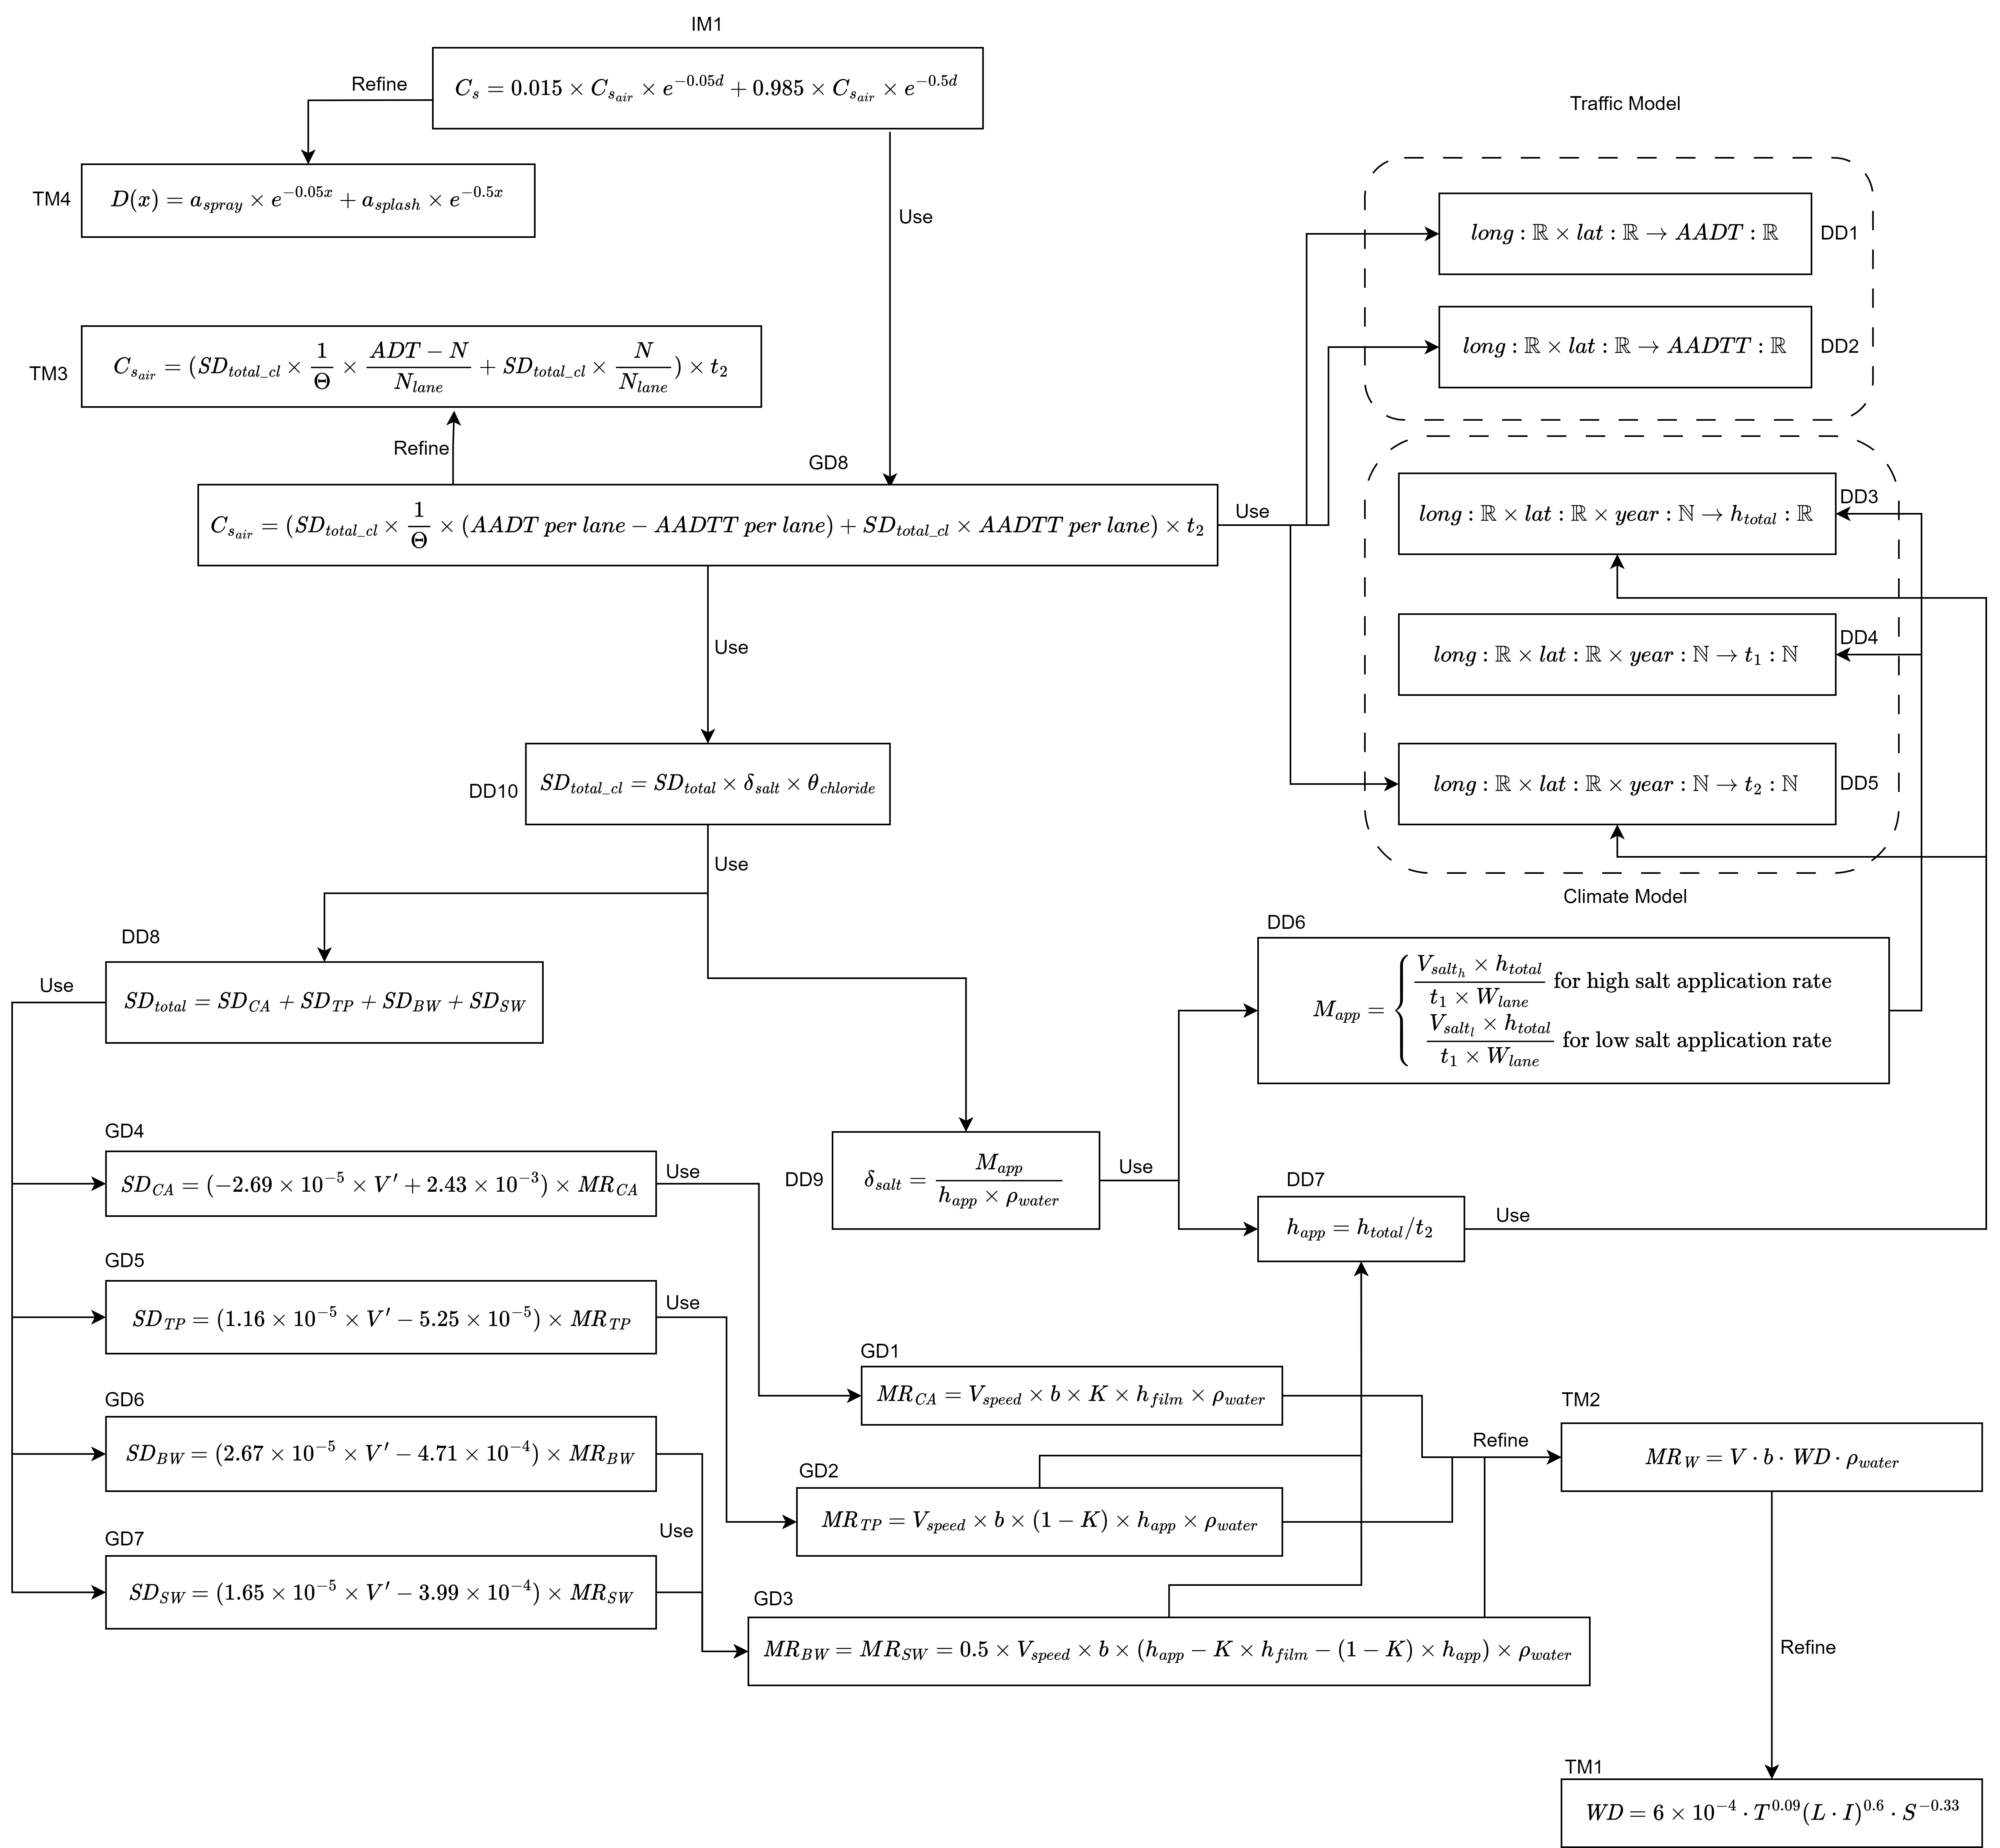
\includegraphics[width=\textwidth]{TraceabilityBetweenModels}
\caption{Traceability Between Models}
\label{Fig_TraceabilityBetweenModels} 
\end{center}
\end{figure}

\noindent
\begin{table}[H]
\centering
\begin{tabular}{|c|c|c|c|c|c|c|c|c|c|c|c|c|c|}
\hline
	& \aref{A_dissolve} & \aref{A_buildup} & \aref{A_pier} & \aref{A_deicingSalts}& \aref{A_laneWidth}& \aref{A_NaCl} & \aref{A_tireWidth} & \aref{A_Speed} & \aref{A_LinearGrowthTraffic} & \aref{A_Data} & \aref{A_Calibration} & \aref{A_deicingSaltsDeposition} &\aref{A_fourMechanisms}\\
\hline
\tref{T_WFT}       & & & & & & & & &  & & & &  \\ \hline
\tref{T_MFRG}      & & & & & & & X & X & &  & & & \\ \hline
\tref{T_CSASG}        & & & & & & & &  & &  & & &\\ \hline
\tref{T_TAD}        & & &  & & && &  & & && &\\ \hline
\dref{D_MRCA}          & & & & & & & X & X  & &  & & &X \\ \hline
\dref{D_MRTP}          & &  & & && & X & X  & &  & & &X \\ \hline
\dref{D_MRBWSW}          & & & & & & & X & X  & &  & X  & &X\\ \hline
\dref{D_SDCA}            & &  & & && & & X  & &  & & & \\ \hline
\dref{D_SDTP}            & &  & & && & & X  & &  & & & \\ \hline
\dref{D_SDBW}            & &  & & && & & X  & &  && &  \\ \hline
\dref{D_SDSW}            & & & & & & & & X  & &  && &  \\ \hline
\dref{D_CSAS}       & & & & & & & &  & & && & \\ \hline
\ddref{DD_AADT}  & & & & & & & & & X &  && & \\ \hline
\ddref{DD_AADTT}  & & &  & & && &  & X & & & &\\ \hline
\ddref{DD_htotal}  & & &  & & && & & &  && & \\ \hline
\ddref{DD_t1}  & & & &  & & && &  & && & \\ \hline
\ddref{DD_t2}  & & & &  & & && &  & & & &\\ \hline
\ddref{DD_DSQ}    & & && X & X & &   &  & & & & & \\ \hline
\ddref{DD_DWFT}    & &  & & && & & &  & && &\\ \hline
\ddref{DD_TSD}    & &  & & && & & & &  && & \\ \hline
\ddref{DD_RSW}    & & & & & & & & & &  && & \\ \hline
\ddref{DD_SDTCL}    &  & & && & X &  & & & && &\\ \hline
\iref{I_COTS}       & & & & & && & & & & & X & \\ \hline
\iref{I_COTD}       & & & & & & & & &  & && & \\ \hline
\iref{I_DFSB}       & & &  & & && &  & & X & & &\\ \hline
\lcref{LC_laneWidth}     &  & & && X & &  & & &  & && \\ \hline
\lcref{LC_SASC}   & & &  & & && & &  & && & \\ \hline
\lcref{LC_northern} & X &  & & && & & &  & && & \\ \hline
\lcref{LC_salt} & & & & & & & & &  & && & \\ \hline
\lcref{LC_resolution} & & & & & & & & &  & X && & \\ \hline
\lcref{LC_linearRegression}  & & & & & & & & &  & && & \\ \hline
\ulcref{ULC_saltSame}    & & && X & & &  && & & &  &\\ \hline
\ulcref{ULC_NaCl}   & & & & & & X &  & & && &  & \\ \hline

\hline
\end{tabular}
\caption{Traceability Matrix Showing the Connections Between Assumptions and Other Items}
\label{Table:A_others}
\end{table}

\begin{landscape}% Landscape page        
\begin{table}[h]
\centering
\setlength{\tabcolsep}{2pt}
\begin{tabular}{|c|c|c|c|c|c|c|c|c|c|c|c|c|c|c|c|c|c|c|c|c|}
\hline        
	& \tref{T_WFT} & \tref{T_MFRG} & \tref{T_CSASG} & \tref{T_TAD} & \dref{D_MRCA} & \dref{D_MRTP} & \dref{D_MRBWSW} & \dref{D_SDCA} & \dref{D_SDTP} & \dref{D_SDBW} & \dref{D_SDSW} & \dref{D_CSAS}& \ddref{DD_DSQ} & \ddref{DD_DWFT}  &  \ddref{DD_TSD} & \ddref{DD_RSW} &\ddref{DD_SDTCL} & \iref{I_COTS} & \iref{I_COTD}  & \iref{I_DFSB}\\ 
\hline

\tref{T_WFT}       &  & X &  & & &  & &  &  &  &  & & &  &  & &&  & &  \\ \hline
\tref{T_MFRG}     &  X &  &  & & X & X  & X &  &  &  &  & & &  &  & &&  & & \\ \hline
\tref{T_CSASG}     &  &  &  & & &  & &  &  &  &  & X & &  &  & &X&  & &\\ \hline
\tref{T_TAD}       &  & &  & & &  & &  &  &  &  & & &  &  & &&X  & &\\ \hline
\dref{D_MRCA}         &  & X &  & & &  & &  X &  &  &  & & &  &  & &&  & & \\ \hline
\dref{D_MRTP}         &  &  X &  & & &  & &  &X  &  &  & & & X &  & &&  & &  \\ \hline
\dref{D_MRBWSW}        &  & X &  & & &  & &  &  & X  & X & & & X  &  & &&  & & \\ \hline
\dref{D_SDCA}         &  &  &  & & X &  & &  &  &  &  & & &  & X  & &&  & & \\ \hline
\dref{D_SDTP}          &  &  &  & & & X & &  &  &  &  & & &  &  X & &&  & &  \\ \hline
\dref{D_SDBW}          &  &  &  & & &  & X &  &  &  &  & & &  & X & &&  & &\\ \hline
\dref{D_SDSW}           &  &  &  & & &  & X &  &  &  &  & & &  & X & &&  & &  \\ \hline
\dref{D_CSAS}       &  &  & X & & &  & &  &  &  &  &  & &  &  & &X& X & &\\ \hline
\ddref{DD_AADT}    &  &  &  & & &  & &  &  &  &  & X & &  &  & &&  & X & \\ \hline
\ddref{DD_AADTT}    &  &  &  & & &  & &  &  &  &  & X& &  &  & &&  & & \\ \hline
\ddref{DD_htotal}   &  &  &  & & &  & &  &  &  &  & & X & X &  & &&  & X & \\ \hline
\ddref{DD_t1}        &  &  &  & & &  & &  &  &  &  & & X &  &  & &&  & & \\ \hline
\ddref{DD_t2}        &  &  &  & & &  & &  &  &  &  & X & &  X &  & &&  & & \\ \hline
\ddref{DD_DSQ}     &  &  &  & & &  & &  &  &  &  & & &  &  & X &&  & &  \\ \hline
\ddref{DD_DWFT}     &  &  &  & & & X & X &  &  &  &  & & &  &  & X &&  & & \\ \hline
\ddref{DD_TSD}     &  &  &  & & &  & & X & X & X & X & & &  &  & &X&  & & \\ \hline
\ddref{DD_RSW}      &  &  &  & & &  & &  &  &  &  & & X & X &  & &X&  & & \\ \hline
\ddref{DD_SDTCL}    &  &  & X & & &  & &  &  &  &  & X & &  &  X&X &&  & & \\ \hline
\iref{I_COTS}        &  &  &  & X & &  & &  &  &  &  &  X & &  &  & &&  & & X \\ \hline
\iref{I_COTD}        &  &  &  & & &  & &  &  &  &  & & &  &  & &&  & & X \\ \hline
\iref{I_DFSB}       &  &  &  & & &  & &  &  &  &  & & &  &  & &&  X & X & \\ \hline
\hline
\end{tabular}
\caption{Traceability Matrix Showing the Connections Between Items of Different Sections}
\label{Table:A_trace}
\end{table}
 \end{landscape}

\newpage
\begin{table}[H]
\centering
\begin{tabular}{|c|c|c|c|}
\hline 
	& \iref{I_COTS} & \iref{I_COTD} & \iref{I_DFSB}  \\

\hline
\rref{R_InputClimate} & X & X & X \\ \hline
\rref{R_InputTraffic} & X & X & X \\ \hline
\rref{R_InputMap} & & & X  \\ \hline
\rref{R_Inputs}     & & & X \\ \hline
\rref{R_Parameter} & X & X &  \\ \hline
\rref{R_OutputInputs} & X  &X & \\ \hline
\rref{R_OutputVisualization} & & & X\\ \hline
\rref{R_OutputDownload} &  & & X\\ \hline
\nfrref{NFR_Reliability}   & X & X & X \\ \hline
\nfrref{NFR_Usability}   & & & X \\ \hline
\nfrref{NFR_Maintainability}   & & & X \\ \hline
\nfrref{NFR_Portability}   & & & X \\ \hline
\nfrref{NFR_Scalability}   & & & X \\
\hline
\end{tabular}
\caption{Traceability Matrix Showing the Connections Between Requirements and Instance Models}
\label{Table:R_trace}
\end{table}


\newpage
\section*{Reference}
\begin{enumerate}[label={[\arabic*]}]
\item \refstepcounter{refnum} \label{ref1}
Smith, W. Spencer and Koothoor, Nirmitha. "A Document-Driven Method for Certifying Scientific Computing Software for Use in Nuclear Safety Analysis." Nuclear Engineering and Technology, vol. 48, no. 2, April, 2016. http://www.sciencedirect.com/-\\science/article/pii/S1738573315002582. pp. 404–418.

\item \refstepcounter{refnum} \label{ref2}
Smith, W. Spencer and Lai, Lei. "A new requirements template for scientific computing." Proceedings of the First International Workshop on Situational Requirements Engineering Processes - Methods, Techniques and Tools to Support Situation-Specific Requirements Engineering Processes, SREP'05. Edited by PJ Agerfalk, N. Kraiem, and J. Ralyte, Paris, France: 2005. pp. 107–121. In conjunction with 13th IEEE International Requirements Engineering Conference

\item \refstepcounter{refnum} \label{ref3}
Smith, W. Spencer, Lai, Lei, and Khedri, Ridha. "Requirements Analysis for Engineering Computation: A Systematic Approach for Improving Software Reliability." Reliable Computing, Special Issue on Reliable Engineering Computation, vol. 13, no. 1, February, 2007. https://doi.org/10.1007/s11155-006-9020-7. pp. 83–107.

\item \refstepcounter{refnum} \label{ref4}
Hanmin Wang, Ravi Ranade \& Pinar Okumus (2023) Estimating chloride exposure of reinforced concrete bridges using vehicle spray and splash mechanisms, Structure and Infrastructure Engineering, 19:11, 1676-1686, DOI: 10.1080/15732479.2022.2052910

\item \refstepcounter{refnum} \label{ref5}
Flintsch, G. W., Tang, L., Katicha, S. W., de Leon Izeppi, E., Viner, H., Dunford, A., ... Gibbons, R. B. (2014). Splash and spray assessment tool development program. Washington, D.C.: Federal Highway Administration.

\item \refstepcounter{refnum} \label{ref6}
Weyers, R. E., Fitch, M. G., Larsen, E. P., Al-Qadi, I. L., Chamberlin, W. P., and Hoffman, P.  C. 1994. Concrete bridge protection and rehabilitation: Chemical and physical techniques. Service life estimates (No. SHRP-S-668).

\item \refstepcounter{refnum} \label{ref7}
Mingsai Xu, Yuxin Zheng, Cancan Yang (2024). Assessing Highway Bridge Chloride Exposure at a Provincial Scale: Mapping and Projecting Impacts of Climate Change.  [Manuscript in preparation].

\item \refstepcounter{refnum} \label{ref8}
Denby, B. R., Sundvor, I., Johansson, C., Pirjola, L., Ketzel, M., Norman, M., ... and Omstedt, G. 2013. “A coupled road dust and surface moisture model to predict non-exhaust road traffic induced particle emissions (NORTRIP). Part 2: Surface moisture and salt impact modelling.” Atmospheric Environment, 81: 485-503, Wang, H., Ranade, R., and Okumus, P. 2022. “Estimating chloride exposure of reinforced concrete bridges using vehicle spray and splash mechanisms.”Structure and Infrastructure Engineering, 1-11. 

\item \refstepcounter{refnum} \label{ref9}
Lysbakken, K. R. (2013). Salting of winter roads: the quantity of salt on road surfaces after application (PhD dissertation). Norwegian University of Science and Technology, Norway.

\item \refstepcounter{refnum} \label{ref10}
Lindvall, A. 2003. Environmental actions on concrete exposed in marine and road environments and its response–Consequences for the initiation of chloride induced reinforcement corrosion (PhD dissertation). Chalmers University of Technology, Gothenburg, Sweden.

\item \refstepcounter{refnum} \label{ref11}
Lundmark, A., and Olofsson, B. 2007. “Chloride deposition and distribution in soils along a deiced highway–assessment using different methods of measurement.” Water, Air, and Soil Pollution, 182: 173-185.

\item \refstepcounter{refnum} \label{ref12}
Blomqvist, G. 2001. De-icing salt and the roadside environment: Air-borne exposure, damage to Norway spruce and system monitoring (PhD dissertation). Institutionen för anläggning och miljö.

\item \refstepcounter{refnum} \label{ref13}
Scinocca, J. F., Kharin, V. V., Jiao, Y., Qian, M. W., Lazare, M., Solheim, L., Flato, G. M., Biner,  S., Desgagne, M., and Dugas, B. 2016. “Coordinated Global and Regional Climate Modeling.” Journal of Climate, 29(1): 17-35.


\end{enumerate}


\end{document}